\section{Application of probabilistic catalogs for population studies}
\lb{sec:pop_studies}

\subsection{Number of sources as a function of flux}
\lb{sec:dNdS}


In this section we show how probabilistic catalogs can be used, for instance, for population studies.
One of the most important questions in gamma-ray astronomy is contribution of point sources, 
e.g., AGNs, to the extragalactic gamma-ray flux 
\citep[e.g.,][]{2010ApJ...720..435A, 2011ApJ...738..181M, 2016PhRvL.116o1105A, 2016ApJS..225...18Z, 2016ApJ...826L..31Z, 2016ApJ...832..117L, 2018ApJ...856..106D}:
if most of the extra-galactic emission is explained by point sources, then one can put stringent constraints, 
e.g., on  dark matter annihilation or decay into gamma rays 
\citep{2015ApJ...800L..27A, 2015PhRvD..91l3001D, 2015JCAP...09..008F, 2015PhR...598....1F, 2017ChPhC..41d5104L} or 
on evaporation of primordial black holes \citep{2010PhRvD..81j4019C}.
In particular, it is important to understand the contribution to the population of AGNs from the unassociated sources.
A probabilistic catalog provides an answer to the question: how many sources among the unassociated ones are expected to belong to different classes, such as pulsars or AGNs. 
One can calculate the total expected number of AGNs or pulsars among the unassociated sources, or calculate the contribution as a function of one or more parameters.
In this subsection we determine the numbers of AGNs and pulsars as a function of their flux, in the following subsection we also discuss the distributions of sources as functions
of Galactic latitude and longitude.



\begin{figure*}[h]
\center
%\hspace*{-1cm}
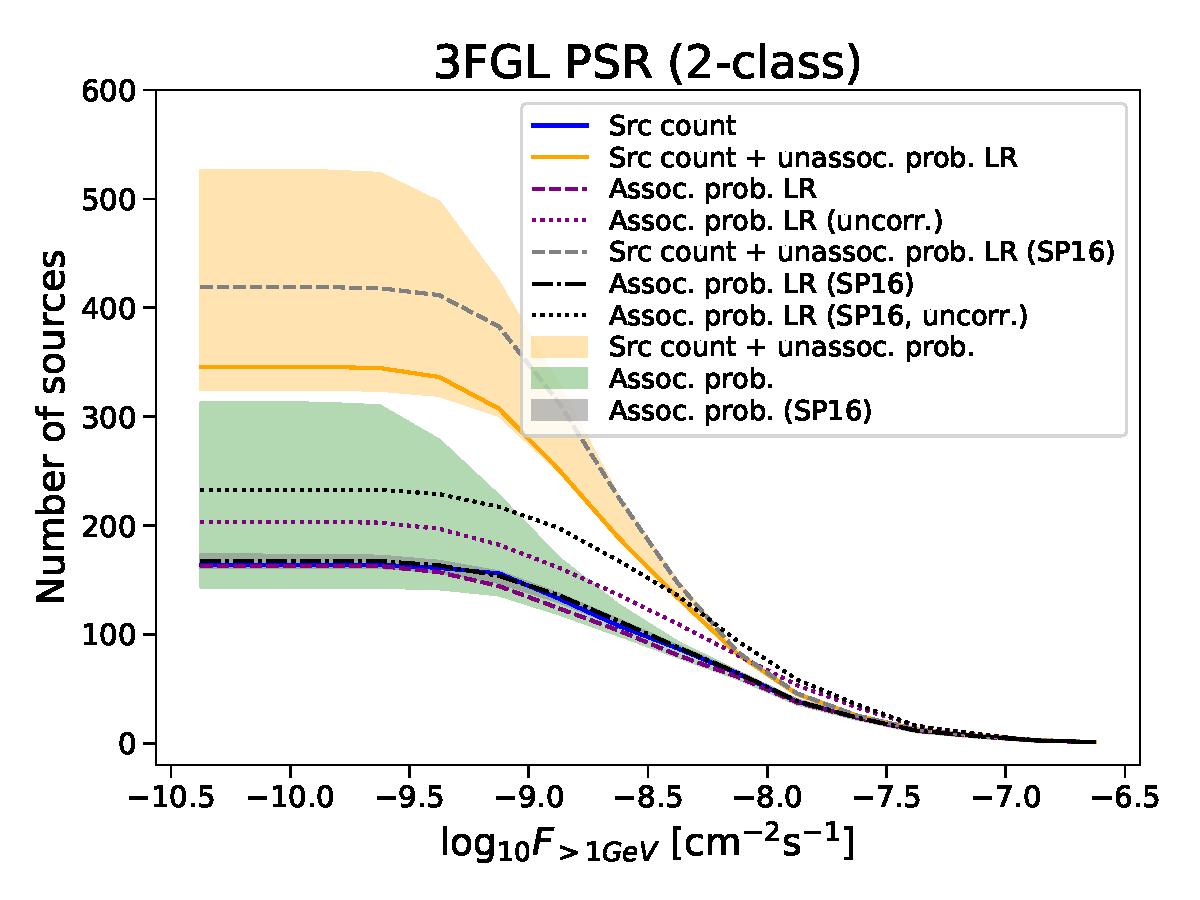
\includegraphics[width=0.45\textwidth]{plots/N_logS_3FGL_PSR_SazP_add_os.pdf}
%\hspace*{-1cm}
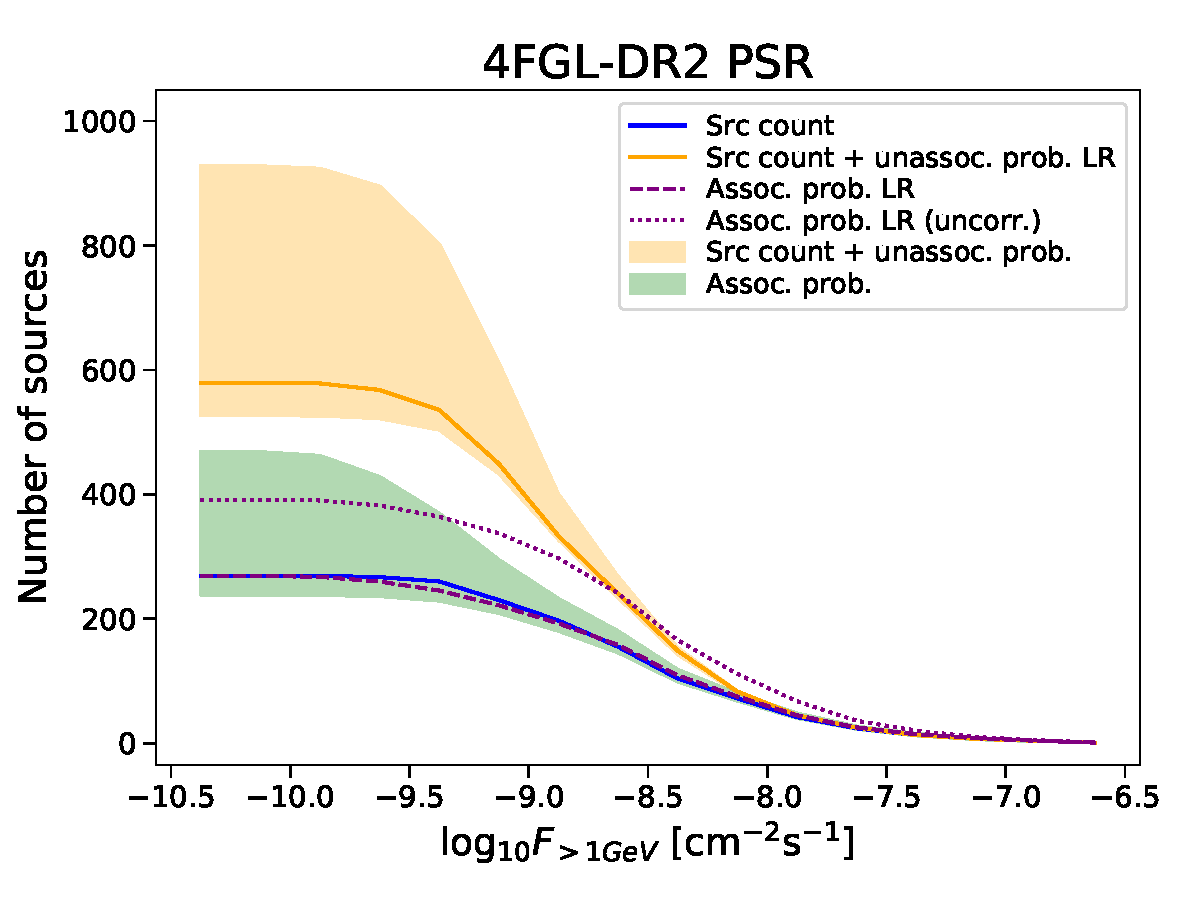
\includegraphics[width=0.45\textwidth]{plots/N_logS_4FGL-DR2_PSR_add_os.pdf} \\
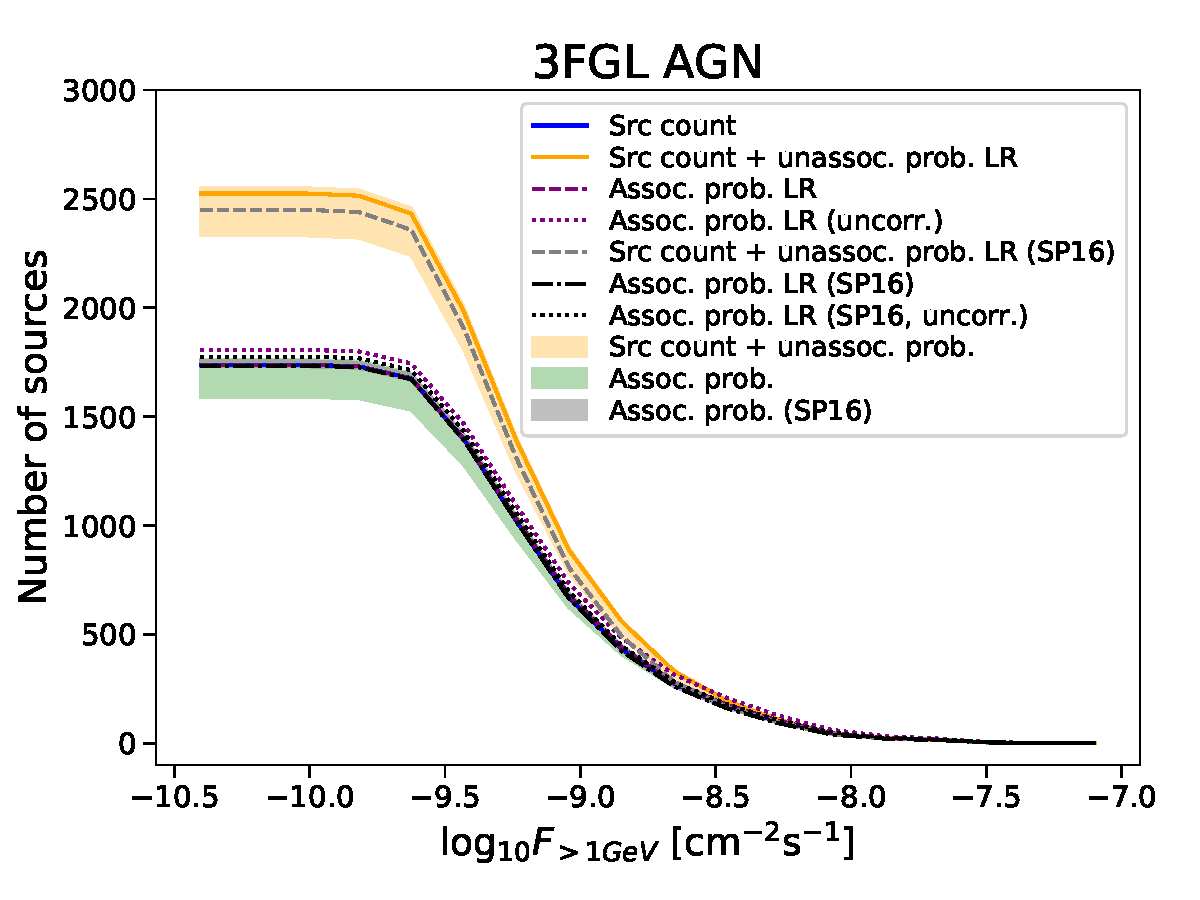
\includegraphics[width=0.45\textwidth]{plots/N_logS_3FGL_AGN_SazP_add_os.pdf}
%\hspace*{-1cm}
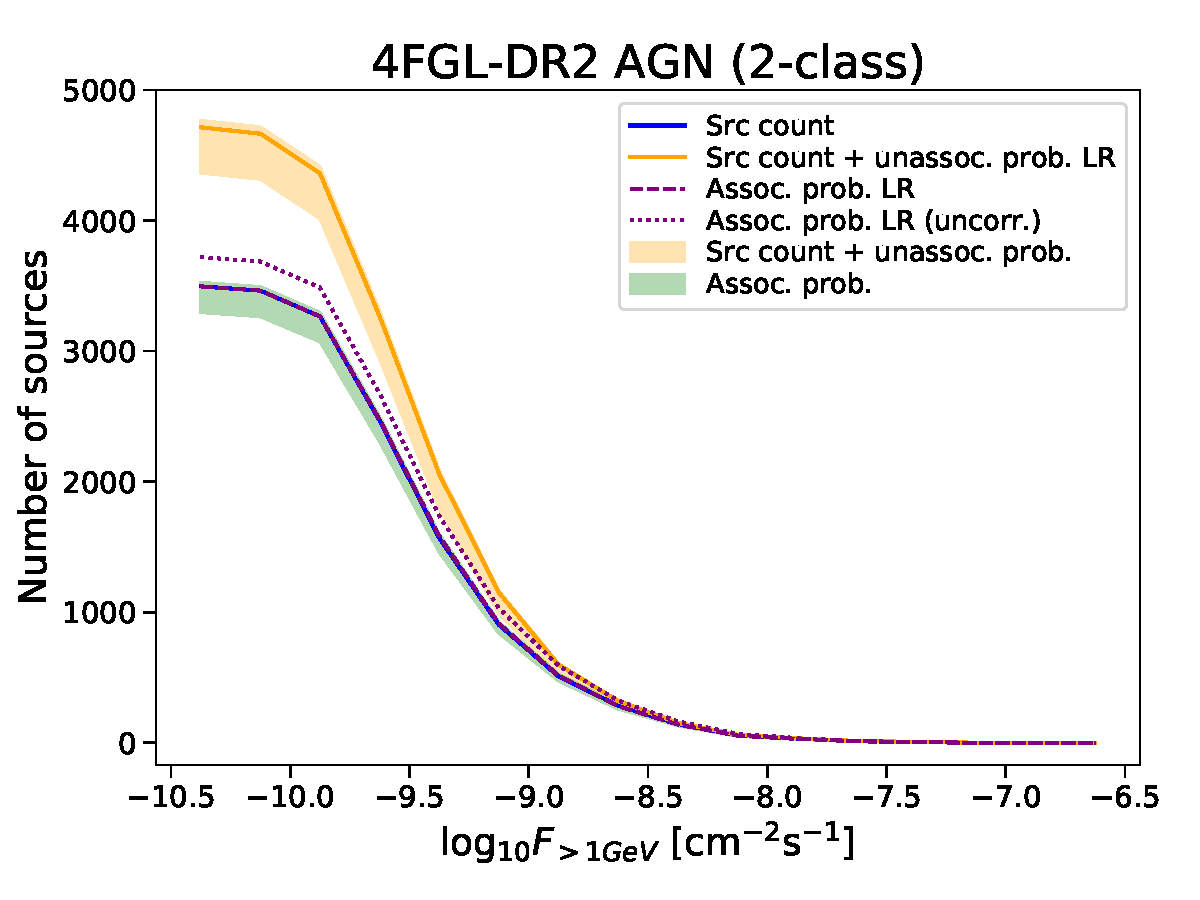
\includegraphics[width=0.45\textwidth]{plots/N_logS_4FGL-DR2_AGN_add_os.pdf}
\caption{Cumulative number of sources as a function of their flux. Green bands show the envelope of the sum of class probabilities for associated sources, while orange bands show the sum of counts of associated sources (blue solid line) plus the sum of probabilities for unassociated sources. The curves with ``SP16'' in the labels are derived from the data in \cite{2016ApJ...820....8S}. For details see Section \ref{sec:dNdS}.}  
\label{fig:logN_logS}
\end{figure*}


\begin{figure*}[h]
\center
%\hspace*{-1cm}
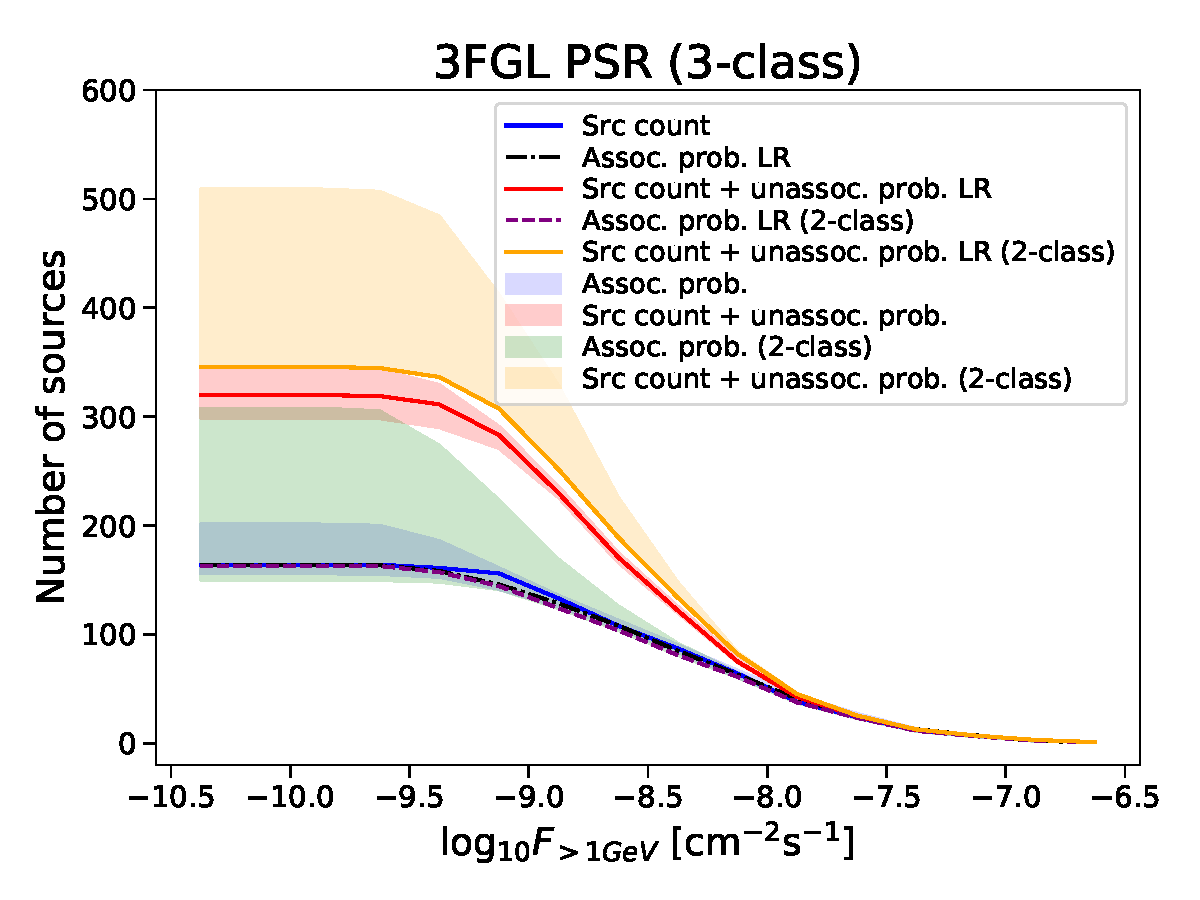
\includegraphics[width=0.45\textwidth]{plots/N_logS_3FGL_PSR_3classes.pdf}
%\hspace*{-1cm}
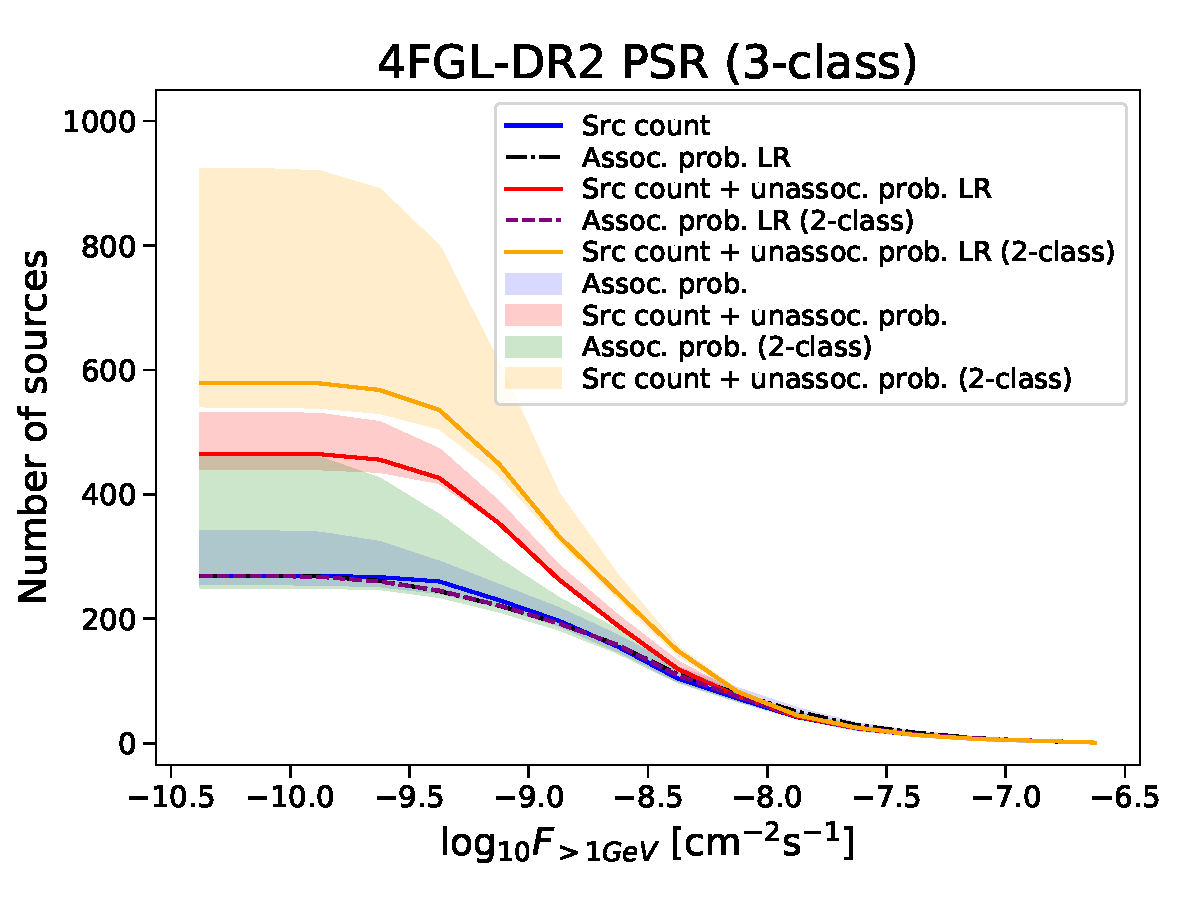
\includegraphics[width=0.45\textwidth]{plots/N_logS_4FGL-DR2_PSR_3classes.pdf} \\
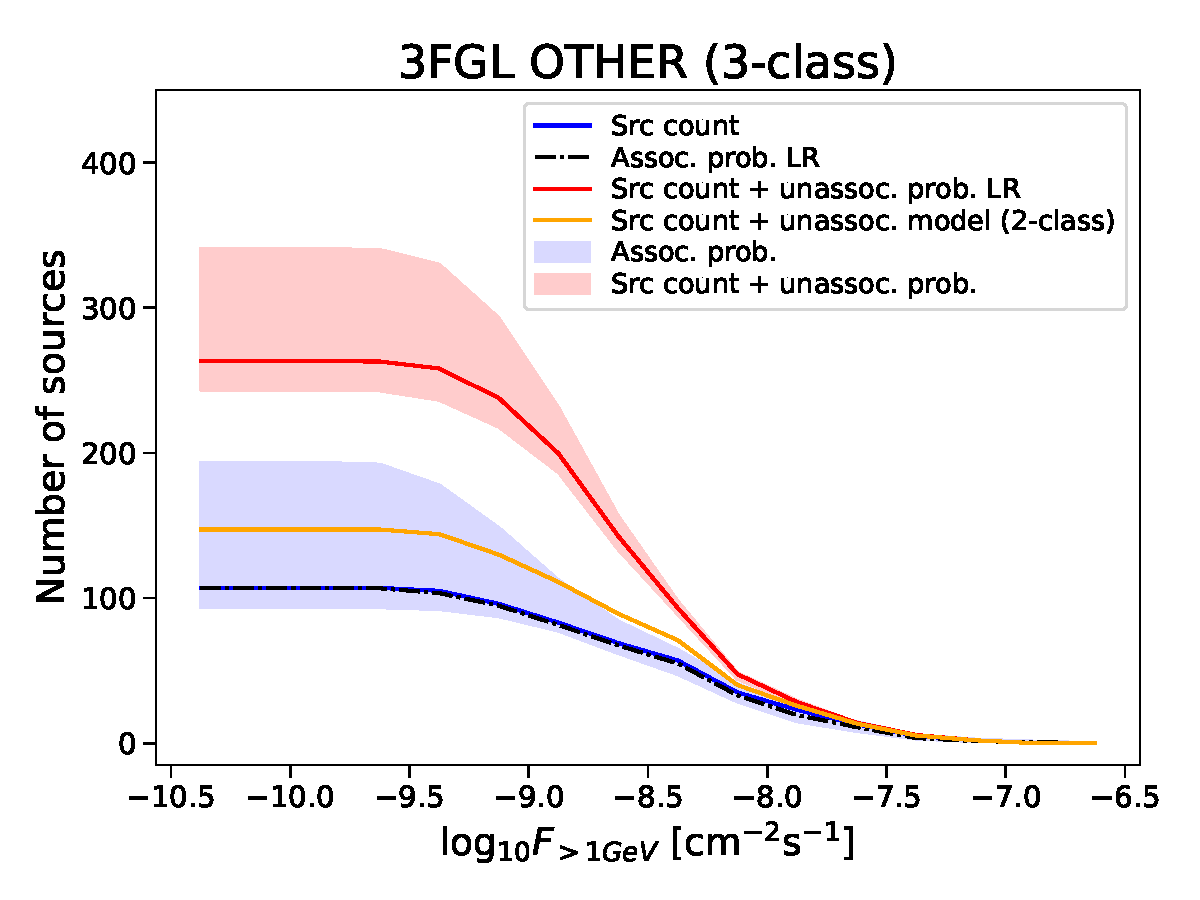
\includegraphics[width=0.45\textwidth]{plots/N_logS_3FGL_OTHER_3classes.pdf}
%\hspace*{-1cm}
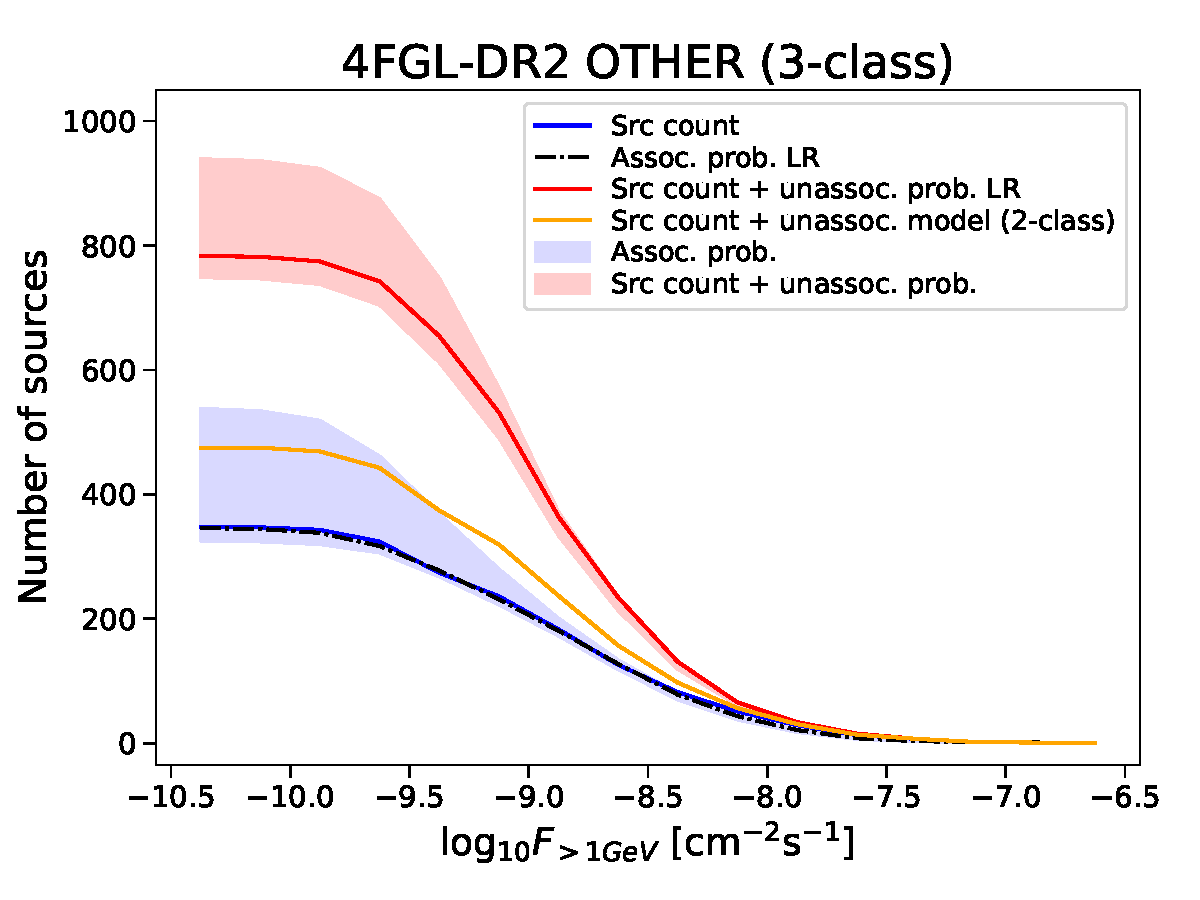
\includegraphics[width=0.45\textwidth]{plots/N_logS_4FGL-DR2_OTHER_3classes.pdf}
\caption{Cumulative number of sources as a function of their flux. Green bands show the envelope of the sum of class probabilities for associated sources, while orange bands show the sum of counts of associated sources (blue solid line) plus the sum of probabilities for unassociated sources. The curves with ``SP16'' in the labels are derived from the data in \cite{2016ApJ...820....8S}. For details see Section \ref{sec:dNdS}.}  
\label{fig:logN_logS_3classes}
\end{figure*}



\begin{figure}[h]
\center
%\hspace*{-1cm}
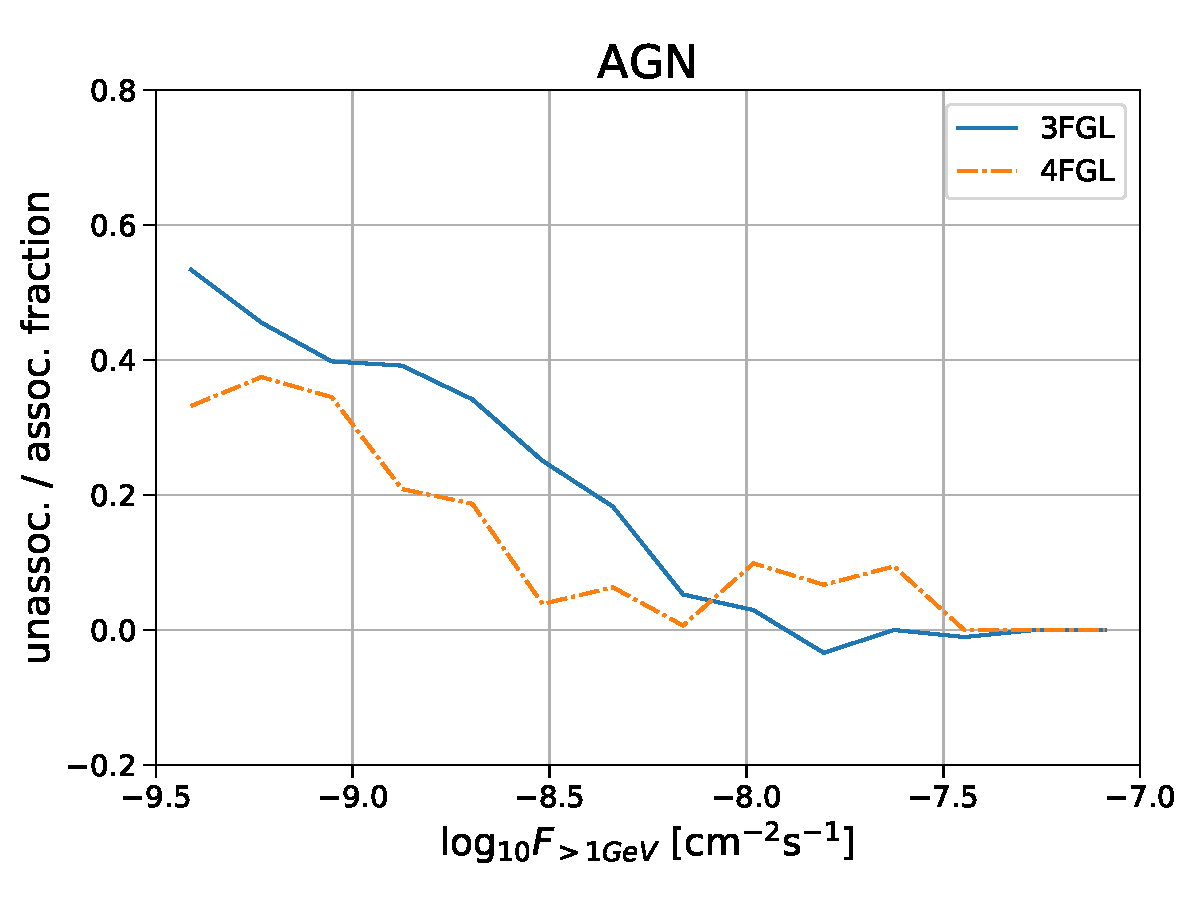
\includegraphics[width=0.45\textwidth]{plots/N_logS_diff_AGN.pdf}
%\hspace*{-1cm}
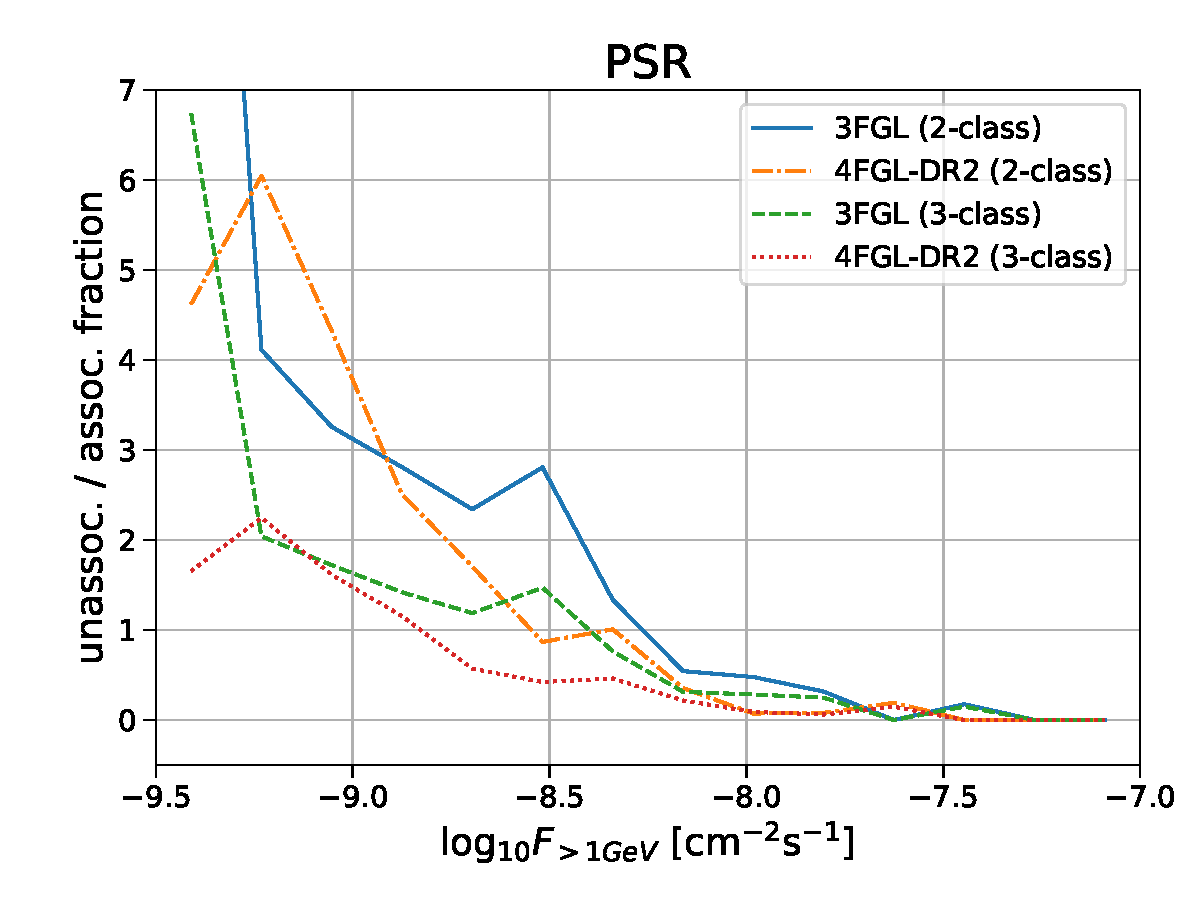
\includegraphics[width=0.45\textwidth]{plots/N_logS_diff_PSR.pdf}
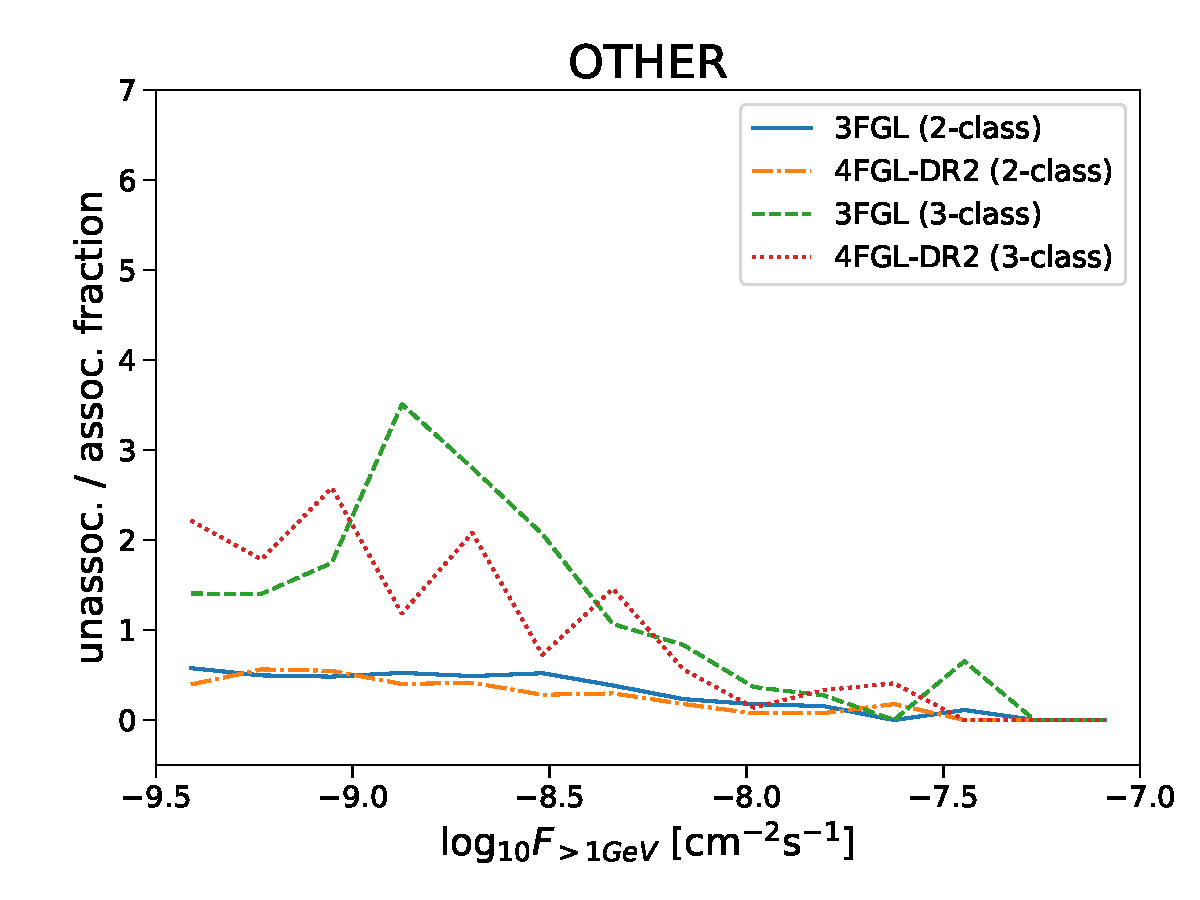
\includegraphics[width=0.45\textwidth]{plots/N_logS_diff_OTHER.pdf}
\caption{Ratio of estimated number of AGNs and pulsars among unassociated sources corrected for the presence of other sources (Equation (\ref{eq:unassoc_ev})) to the counts of associated AGNs and pulsars respectively.}  
\label{fig:unass_vs_ass_frac}
\end{figure}




In Figure \ref{fig:logN_logS} we show the cumulative number of AGNs and pulsars with flux above 1 GeV larger than the
value on the x-axis.
Solid blue lines show the actual counts of sources (AGNs or pulsars) in the 3FGL and 4FGL-DR2 catalogs.
As a consistency check of the method, we calculate the AGN- and PSR-like probabilities for associated sources.
The sum of probabilities (uncorrected for sources other than AGNs and pulsars) for LR algorithm are shown by dotted purple lines.
In order to correct the expected number of AGNs among associated sources for AGN-like probabilities in ``other'' sources, 
we subtract the corresponding AGN-like probabilities in each flux band:

\be
\lb{eq:assoc_ev}
N_{\rm AGN}^{\rm ass}  = \sum_{i \in \rm ass} p^i_{\rm AGN}\,\, - \sum_{i \in \rm ass\,other} p^i_{\rm AGN}.
\ee
The corrected sums of probabilities for LR method are shown by dashed purple lines.
The green bands show the envelope of the sums of corrected probabilities for the eight methods used in this paper.
We see that the counts of associated sources, AGNs and pulsars, are consistent with the expected number of associated sources
calculated from the class probabilities of associated sources.
This conclusion is not very surprising since we used associated sources for training of ML algorithms.
It is important to note that correction for ``other'' sources is important for consistency of the sum of probabilities and the number of associated sources.
We have also compared the sums of probabilities for the 3FGL associated sources in \cite{2016ApJ...820....8S}.
%\footnote{The data is downloaded from \url{https://www.physics.hku.hk/~pablo/pulsarness.html}.} !!! resolve the footnote issue?
The sum of probabilities for associated sources in the LR case uncorrected for ``other'' sources are shown by dotted black line,
while the sums corrected for ``other'' sources are shown by black dash-dotted lines.
The gray band is the envelope of the two methods (LR and RF) used by \cite{2016ApJ...820....8S}.
We see that the sum of probabilities for pulsars overpredicts the pulsar counts in 3FGL, 
while correction for ``other'' sources makes the prediction consistent with the counts of pulsars.

The predictions for the number of AGNs and pulsars among the unassociated sources corrected for ``other'' sources 
added to the 3FGL and 4FGL-DR2  source counts are shown by solid orange lines (for the LR case).
The orange bands show the corresponding envelopes for the eight ML methods.
We assume that the fractional contribution of other sources is the same for associated and unassociated sources in the different flux bands.
Thus, the correction for the presence of other sources is calculated similarly to the associated sources in Equation \ref{eq:assoc_ev},
but we adjust for the fact that there are fewer unassociated than associated sources, i.e., 
the correction is assumed to be proportionally smaller.
In particular, the number of AGNs among unassociated sources in a flux band $\Delta F$ is estimated as

\be
\lb{eq:unassoc_ev}
N_{\rm AGN}^{\rm unass} = \sum_{i \in \rm unass} p^i_{\rm AGN}\,\, - \sum_{i \in \rm ass\,other} p^i_{\rm AGN} \cdot 
\frac{N_{\rm unass}}{N_{\rm ass}}
\ee
where all probabilities and the numbers of sources are computed for sources with flux inside $\Delta F$.
The first term is the sum of AGN-like probabilities among the unassociated sources,
while the second term is the sum of AGN-like probabilities among associated ``other'' sources rescaled by the total number
of unassociated and associated sources in this flux band.
The expected number of pulsars among the unassociated sources is calculated analogously.
The corresponding sums of associated source counts plus the expected number of sources calculated with LR method of \cite{2016ApJ...820....8S} 
and corrected for other sources are shown by dashed grey lines.


We predict that the expected number of pulsars among the unassociated sources in the 3FGL catalog
is $261 \pm 100$, where the range is the envelop of the sums of probabilities in Equation (\ref{eq:unassoc_ev})
for different ML methods (including oversampling) corrected for other sources among the unassociated sources.
The expected number of pulsars among the unassociated sources in the 4FGL-DR2  catalog corrected for other sources is 
$459 \pm 201$.
These numbers are larger than the number of associated PSRs without missing values (164 in 3FGL and 269 in 4FGL-DR2 ).
Even at the lower range of expected numbers of pulsars among unassociated sources, there are potentially as many pulsars
as there are associated ones.

We note that according to Table \ref{tab:3FGL_prediction}, the number of unassociated 3FGL sources 
with $p_{\rm PSR} > 0.5$ for all four ML algorithms is 111 (97), while there are 300 (279) sources with mixed classification,
uncorrected (corrected) for other sources.
The number of sources with mixed classification (279 for 3FGL or 563 for 4FGL-DR2)
is larger than the range of values for the expected number of pulsars calculated for the sum of probabilities 
(200 for 3FGL or 402 for 4FGL-DR2 ).
It means that the decision which sources are considered to be more likely pulsars is more sensitive to the choice of the ML method
and the probability threshold than the expected number of pulsars calculated from the sum of probabilities.

The numbers of PSRs and OTHER sources as a function of flux are shown in Figure \ref{fig:logN_logS_3classes}.
As in the two-class case, solid blue line shows the counts of associated sources in the corresponding classes.
Red and blue bands show the envelops of the expected number of associated sources and the number of associated sources plus the expected numbers of 
sources among unassociated ones respectively.
In the PSR plots, we also replot the envelops of expected numbers of associated PSR (shown by the green band) and associated source counts plus prediction for unassociated sources by orange bands corrected for the presence of OTHER sources among unassociated ones.
We notice that the bands for the 3-class case are narrower in the PSR plots than the bands for the 2-class case.
In part this is due to less oversampling in the 3-class case. But it is not the only reason: the red band lies almost entirely below the orange one.
This is due to a possible underestimation of the contribution of OTHER sources to the PSR class among unassociated sources.
In particular, on the bottom panels of Figure \ref{fig:logN_logS_3classes} we show the estimated total number of OTHER sources in the 2-class case by the orange line.
Since we do not have probabilities for the OTHER sources in this case, we estimate the number of OTHER sources among unassociated ones 
simply by rescaling the number of associated OTHER sources in each energy band as
\be
\lb{eq:unas_other}
N_{\rm OTHER}^{\rm unass} = N_{\rm OTHER}^{\rm ass} \frac{N^{\rm unass}}{N^{\rm ass}}
\ee
We notice that this estimate agrees with the correction of the estimated numbers of AGNs and pulsars in the 2-class case due to presence of other sources, since
\bea
\nonumber
N_{\rm OTHER}^{\rm ass} &=& \sum_{i \in \rm ass\,other} p^i_{\rm AGN} + \sum_{i \in \rm ass\,other} p^i_{\rm PSR} \\
&=& \sum_{i \in \rm ass\,other} (p^i_{\rm AGN} + p^i_{\rm PSR})
\eea
provided that $p^i_{\rm AGN} + p^i_{\rm PSR} = 1$ for each source in the two-class case.
The estimated total number of OTHER sources in the 2-class case (orange line) is significantly below the red band derived from the sum of probabilities
of the OTHER class in the 3-class case.
\dima{Interpretation of discrepancy with OTHER sources predictions. Refer to a domain plot?}
Both 2-class and 3-class predictions for the number of associated PSRs and AGNs agree with the actual counts of associated PSRs and AGNs.


We note that the probabilistic classification mostly affects sources with small fluxes.
In Figure \ref{fig:unass_vs_ass_frac} we plot the ratio of the expected number of sources of a certain class among unassociated sources
computed according to Eq. \ref{eq:unassoc_ev} with the LR algorithm (without oversampling) to the number of associated sources in this class.
The ratio generally increases as the flux decreases.
Negative values (e.g., at high fluxes for AGNs) are due to subtraction of probabilities for the ``other'' associated sources.



\subsection{Latitude and longitude profiles}
\lb{sec:lat-lon-profiles}

\begin{figure*}[h]
\center
%\hspace*{-1cm}
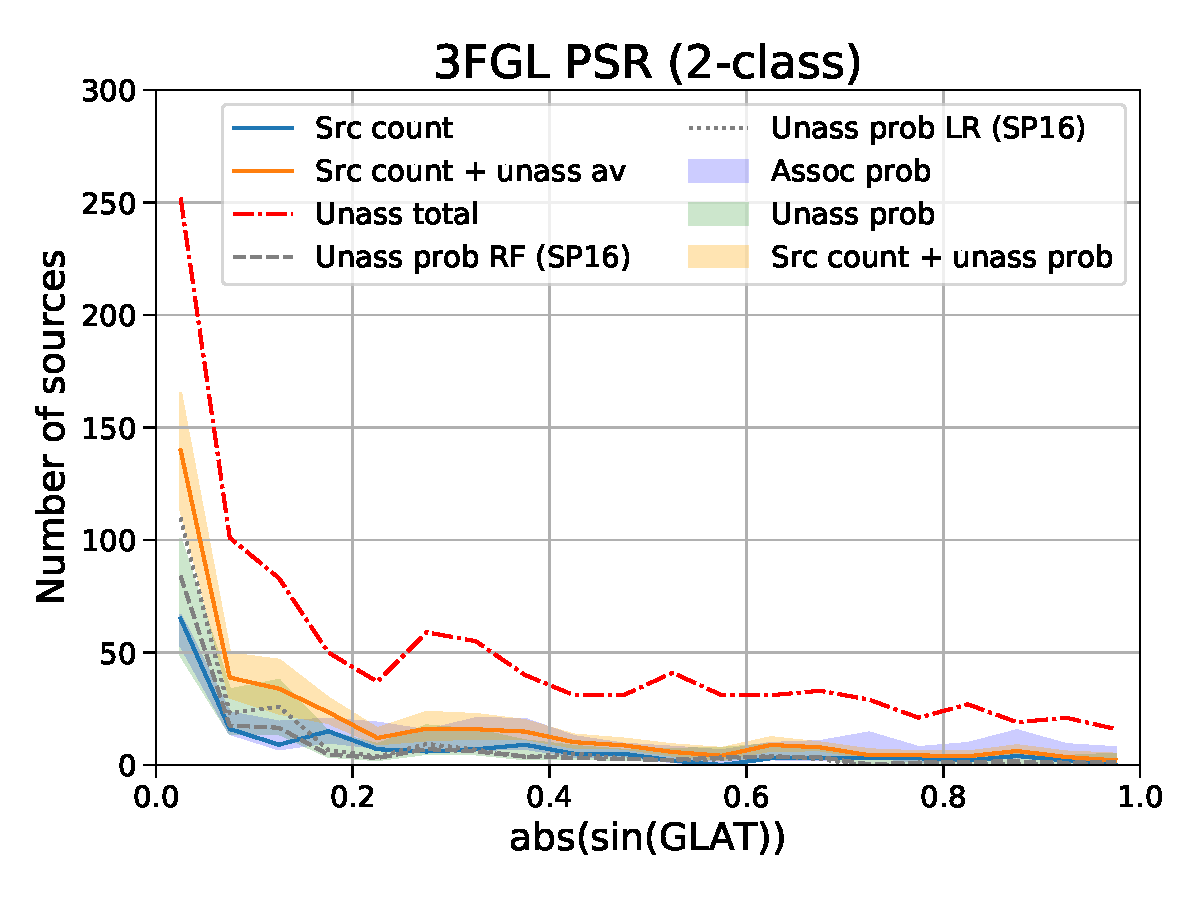
\includegraphics[width=0.45\textwidth]{plots/lat_profile_PSR_3FGL_2classes.pdf}
%\hspace*{-1cm}
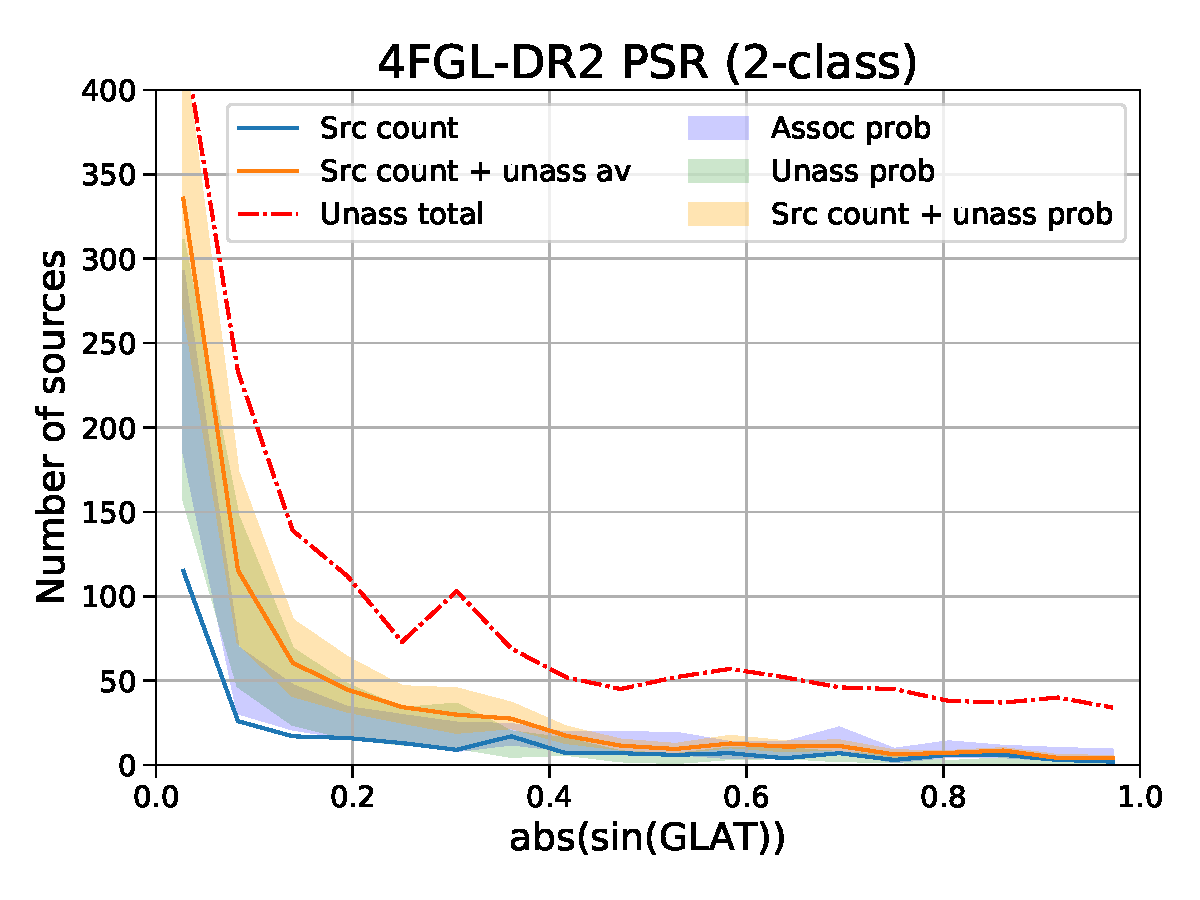
\includegraphics[width=0.45\textwidth]{plots/lat_profile_PSR_4FGL-DR2_2classes.pdf} \\
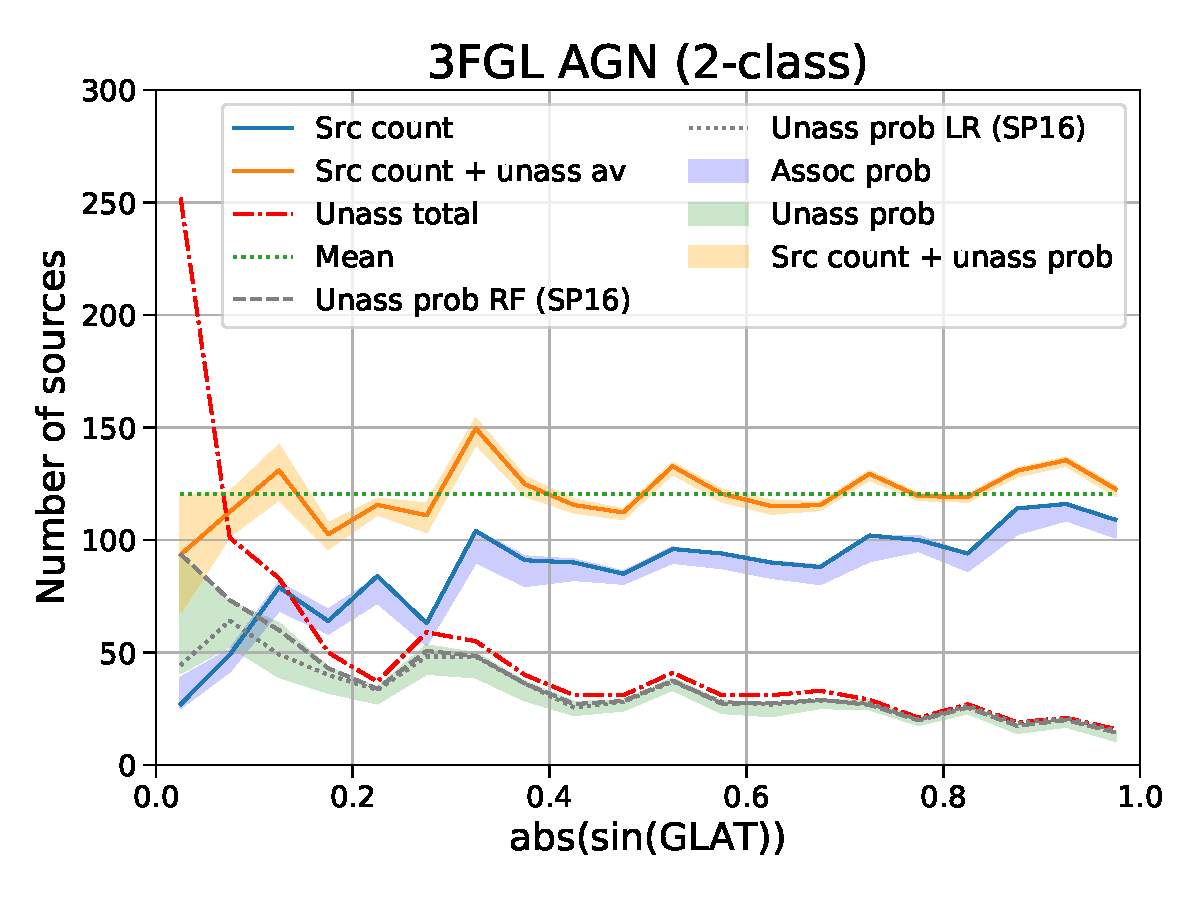
\includegraphics[width=0.45\textwidth]{plots/lat_profile_AGN_3FGL_2classes.pdf}
%\hspace*{-1cm}
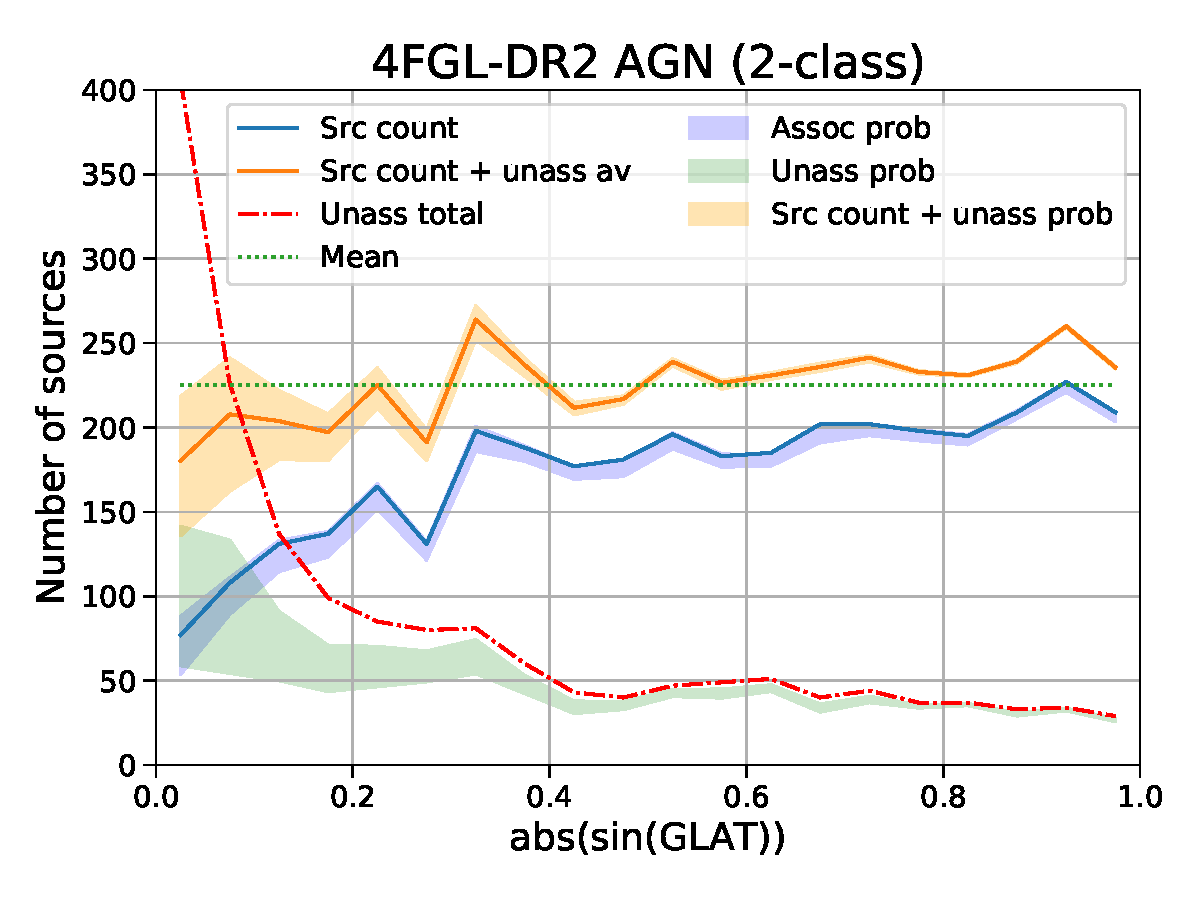
\includegraphics[width=0.45\textwidth]{plots/lat_profile_AGN_4FGL-DR2_2classes.pdf}
\caption{Latitude profiles of source counts in case of 2-class classification. 
Blue solid line -- associated 3FGL and 4FGL-DR2  sources. 
Red dash-dotted line -- counts of all unassociated sources. 
Blue band - envelope of sums of class probabilities for associated sources for the eight ML methods with and without oversampling
corrected for the presence of OTHER sources.
Green band -- envelope of sums of class probabilities for unassociated sources for the eight ML methods corrected for the presence of OTHER sources. 
Orange solid line (band) -- average (envelope) of sums of class probabilities for the eight ML methods added to the source count of associated sources. 
Green dotted line on the AGN plots -- mean of the orange solid line.
Gray dashed (dotted) line -- RF (LR) sums of class probabilities from \cite{2016ApJ...820....8S}.
For details see Section \ref{sec:lat-lon-profiles}. }  
\label{fig:lat_profile}
\end{figure*}

\begin{figure*}[h]
\center
%\hspace*{-1cm}
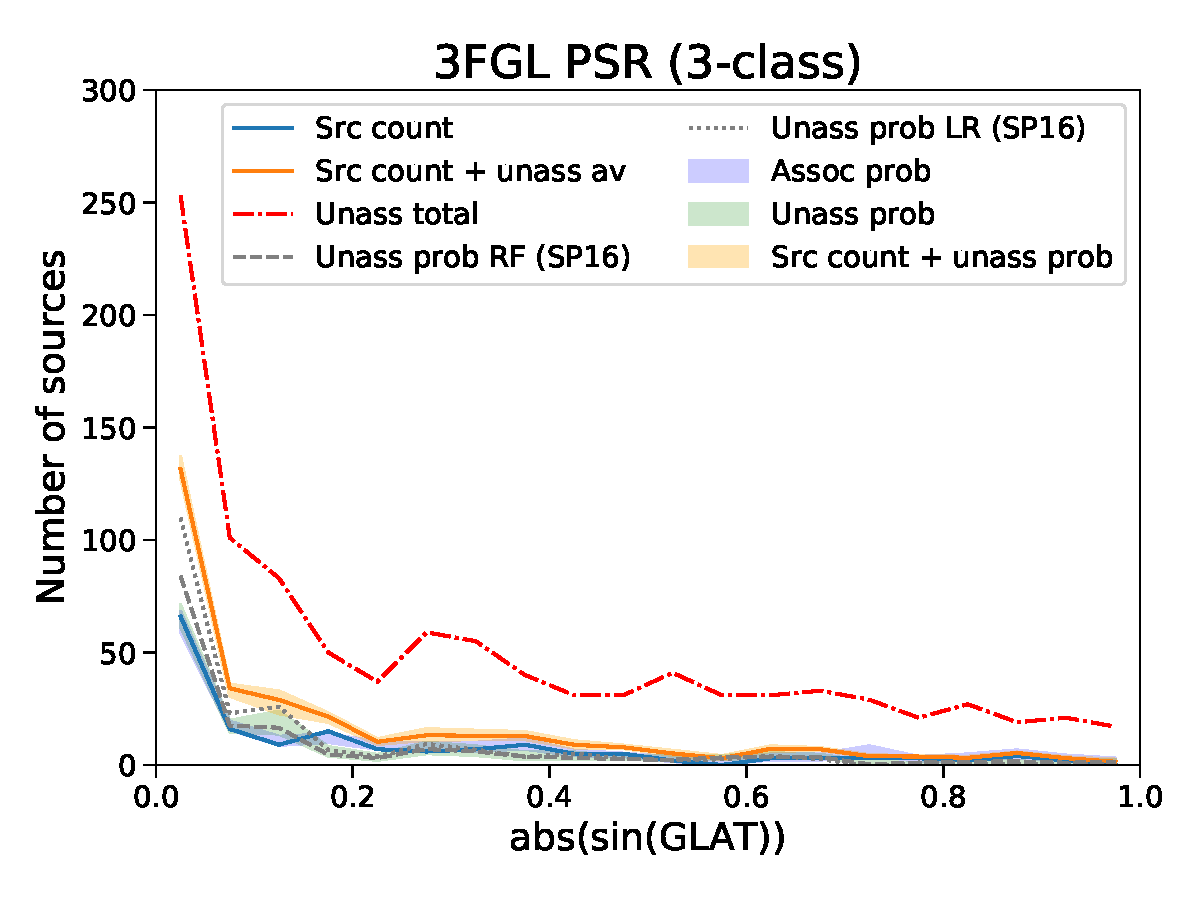
\includegraphics[width=0.45\textwidth]{plots/lat_profile_PSR_3FGL_3classes.pdf}
%\hspace*{-1cm}
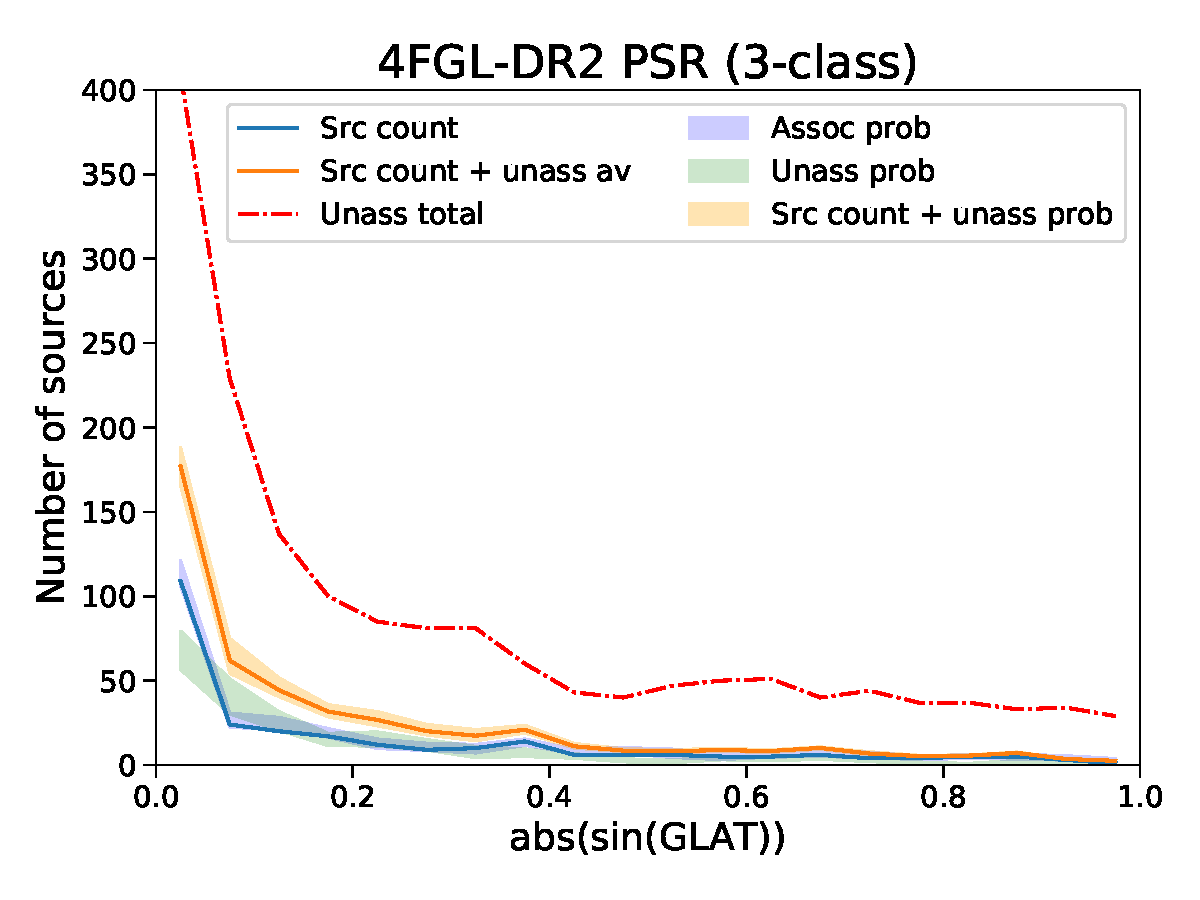
\includegraphics[width=0.45\textwidth]{plots/lat_profile_PSR_4FGL-DR2_3classes.pdf} \\
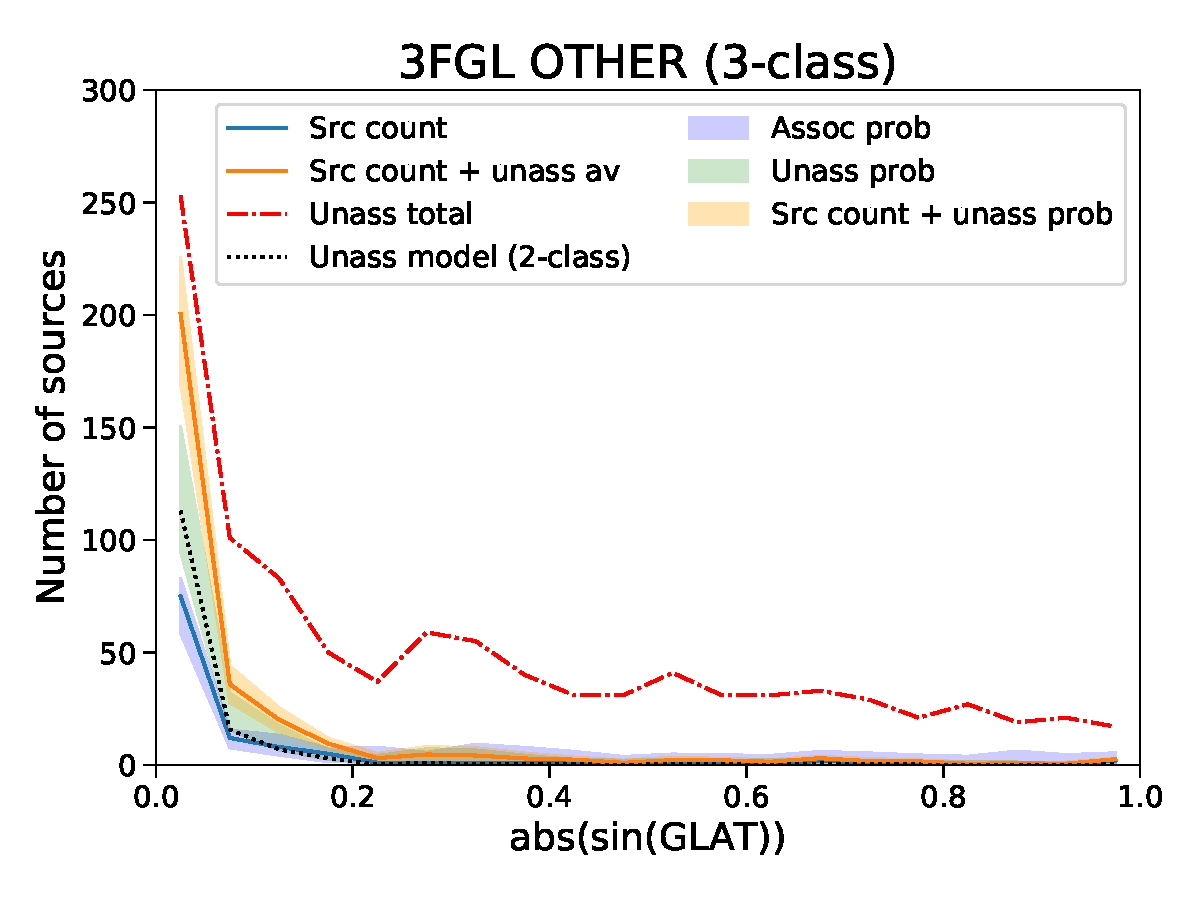
\includegraphics[width=0.45\textwidth]{plots/lat_profile_OTHER_3FGL_3classes.pdf}
%\hspace*{-1cm}
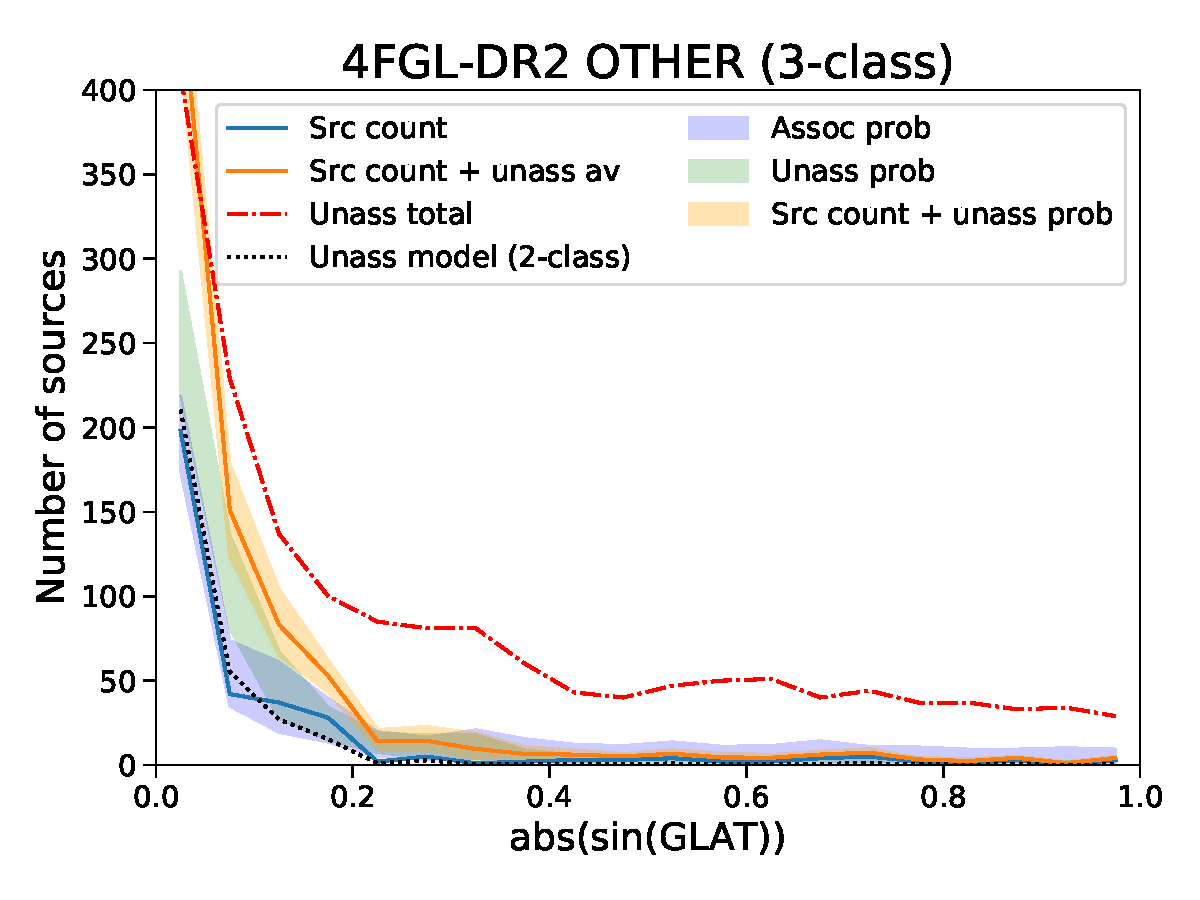
\includegraphics[width=0.45\textwidth]{plots/lat_profile_OTHER_4FGL-DR2_3classes.pdf} \\ 
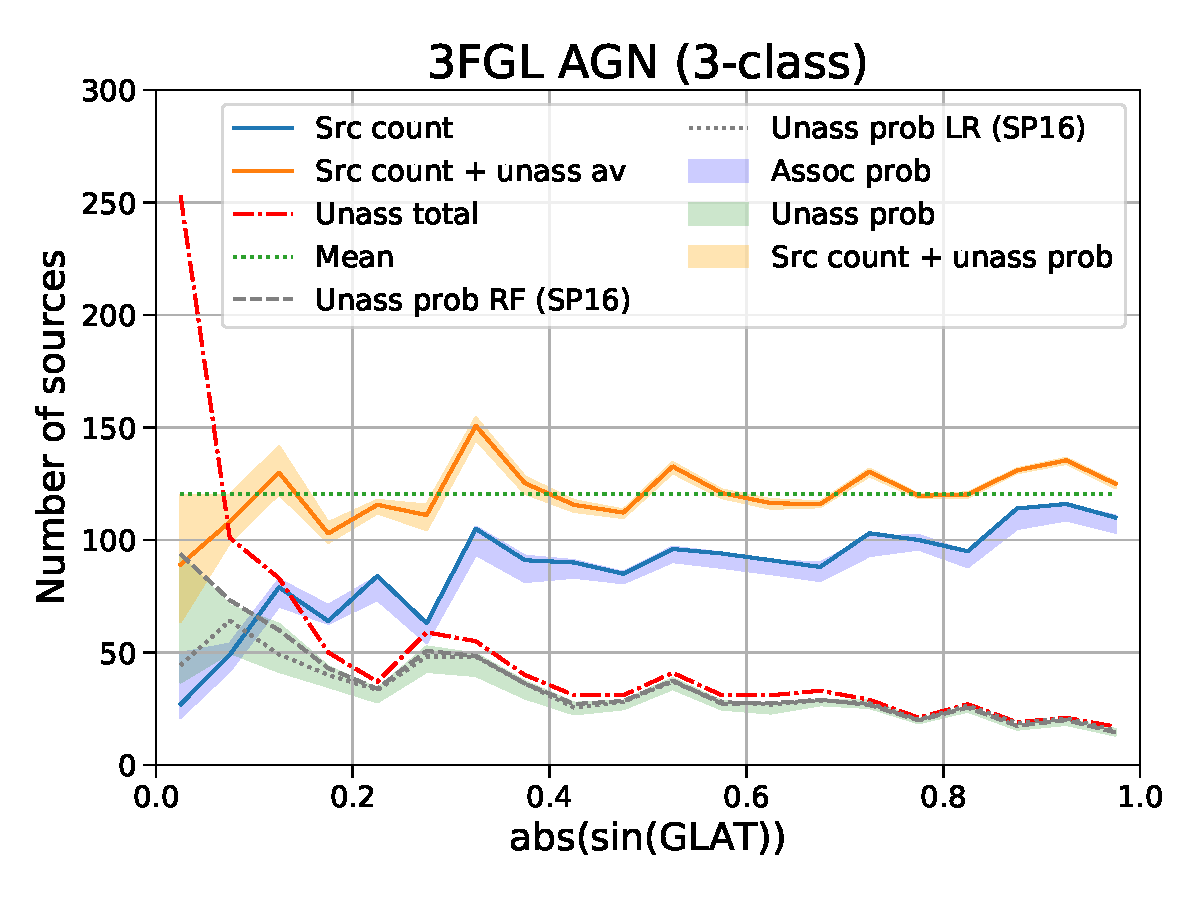
\includegraphics[width=0.45\textwidth]{plots/lat_profile_AGN_3FGL_3classes.pdf}
%\hspace*{-1cm}
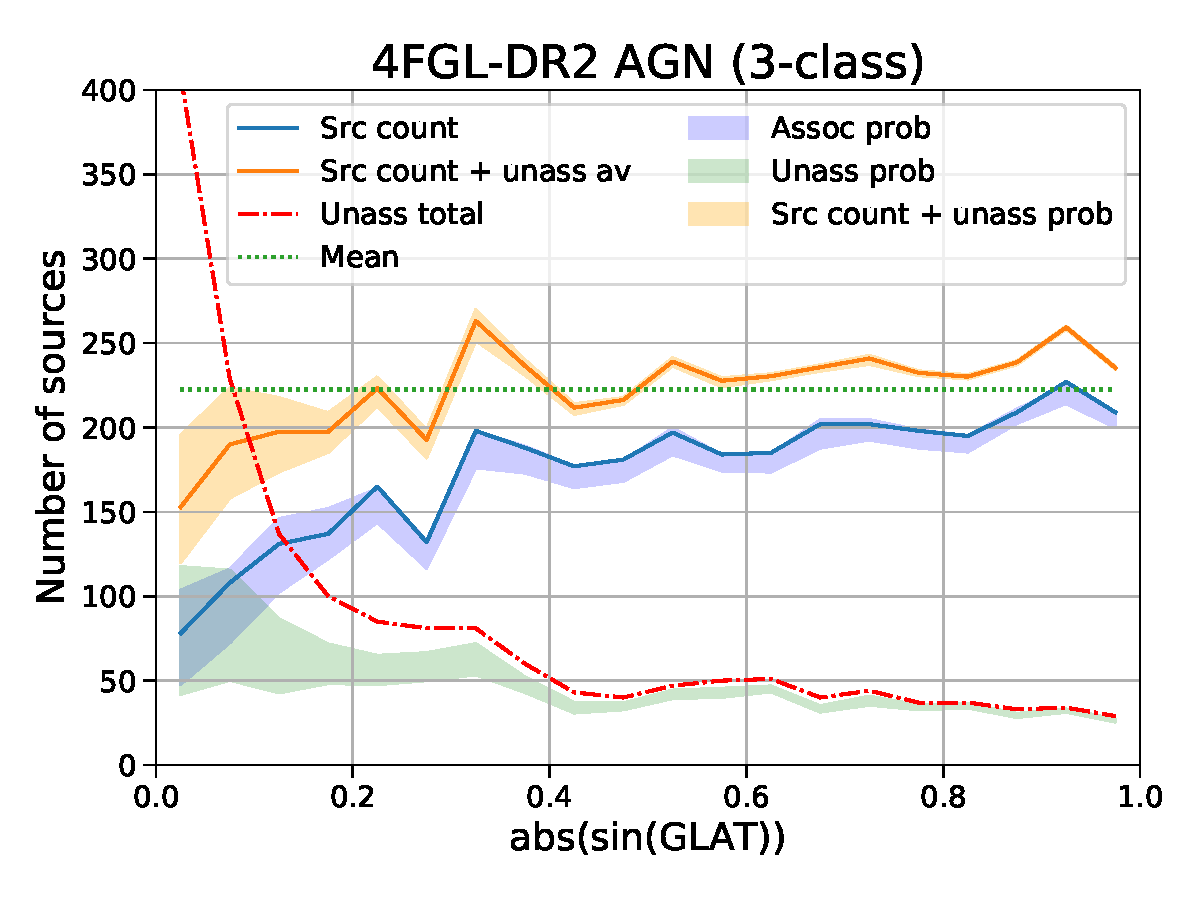
\includegraphics[width=0.45\textwidth]{plots/lat_profile_AGN_4FGL-DR2_3classes.pdf}
\caption{Latitude profiles of source counts in case of 3-class classification. For the definition of labels see Figure \ref{fig:lat_profile}.
Black dashed line in plots of the OTHER class show the model for the number of OTHER sources among the unassociated ones
in Equation (\ref{eq:unas_other}) for latitude bins.}
\label{fig:lat_profile_3class}
\end{figure*}


\begin{figure*}[h]
\center
%\hspace*{-1cm}
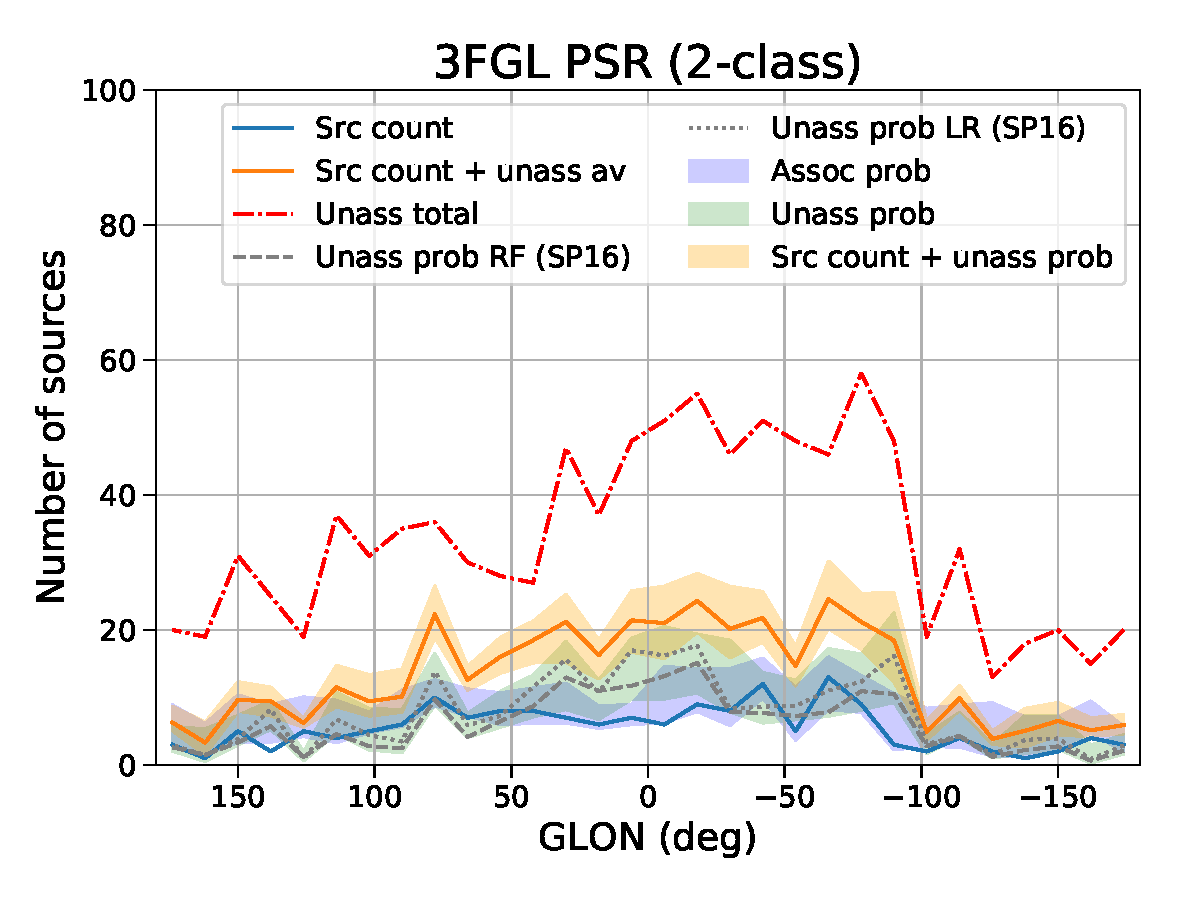
\includegraphics[width=0.45\textwidth]{plots/lon_profile_PSR_3FGL_2classes.pdf}
%\hspace*{-1cm}
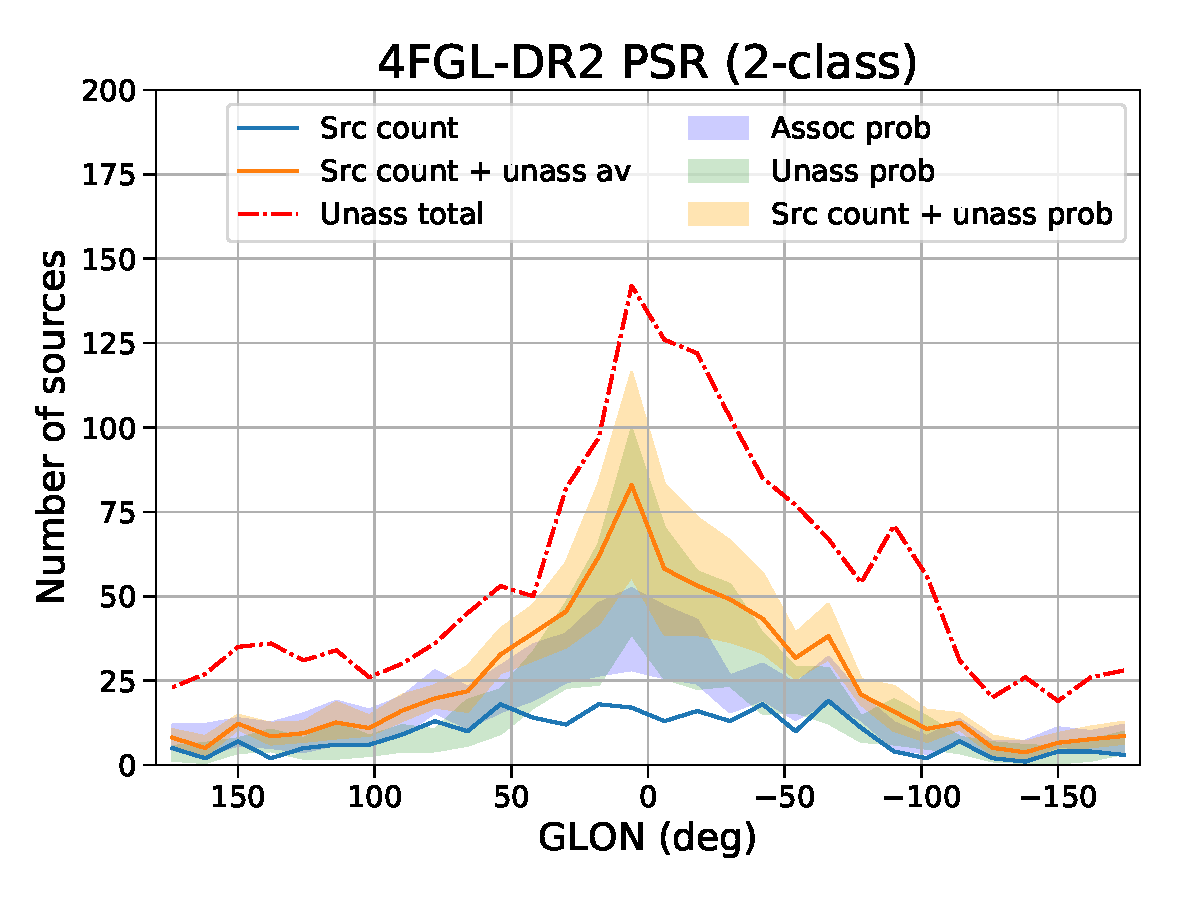
\includegraphics[width=0.45\textwidth]{plots/lon_profile_PSR_4FGL-DR2_2classes.pdf} \\
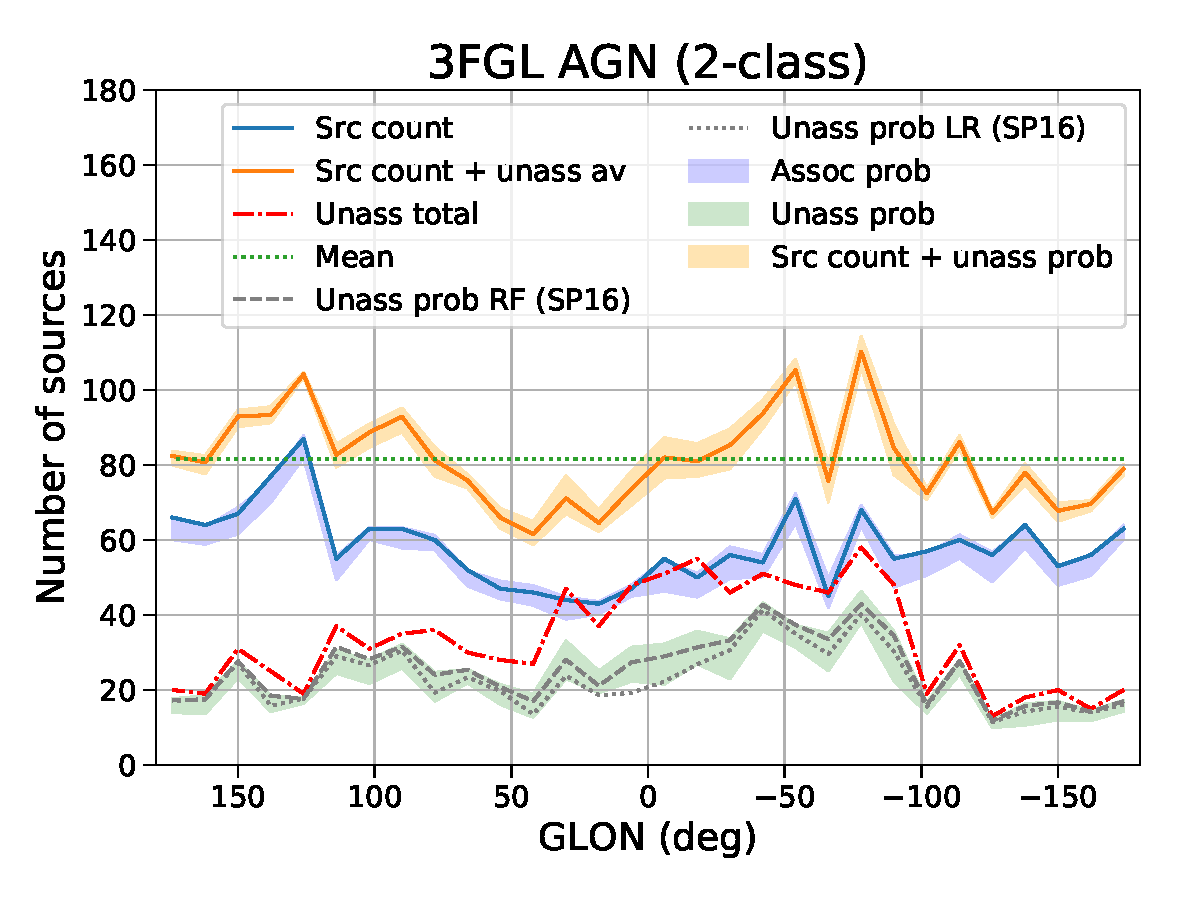
\includegraphics[width=0.45\textwidth]{plots/lon_profile_AGN_3FGL_2classes.pdf}
%\hspace*{-1cm}
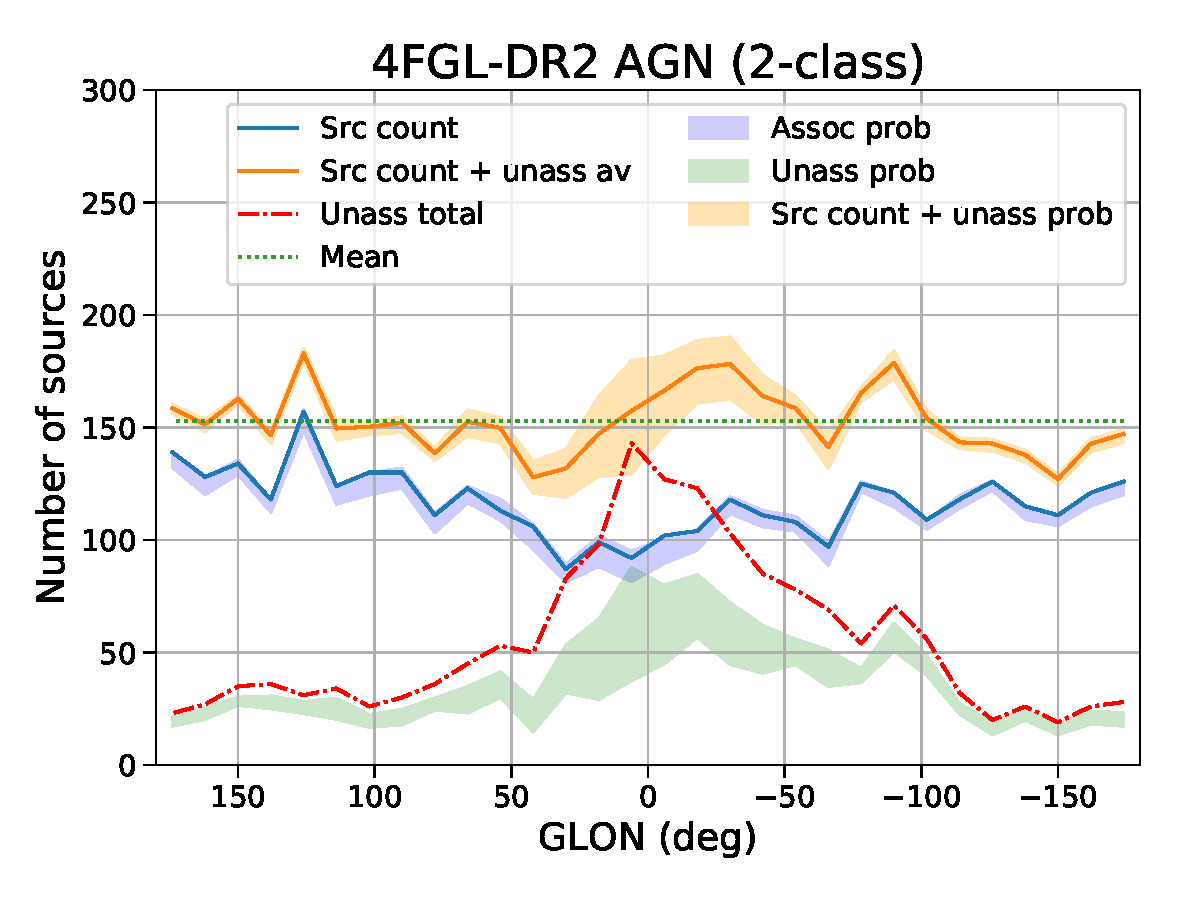
\includegraphics[width=0.45\textwidth]{plots/lon_profile_AGN_4FGL-DR2_2classes.pdf}
\caption{Longitude profiles of source counts in case of 2-class classification. For the definition of labels see Figure \ref{fig:lat_profile}.}  
\label{fig:lon_profile}
\end{figure*}



\begin{figure*}[h]
\center
%\hspace*{-1cm}
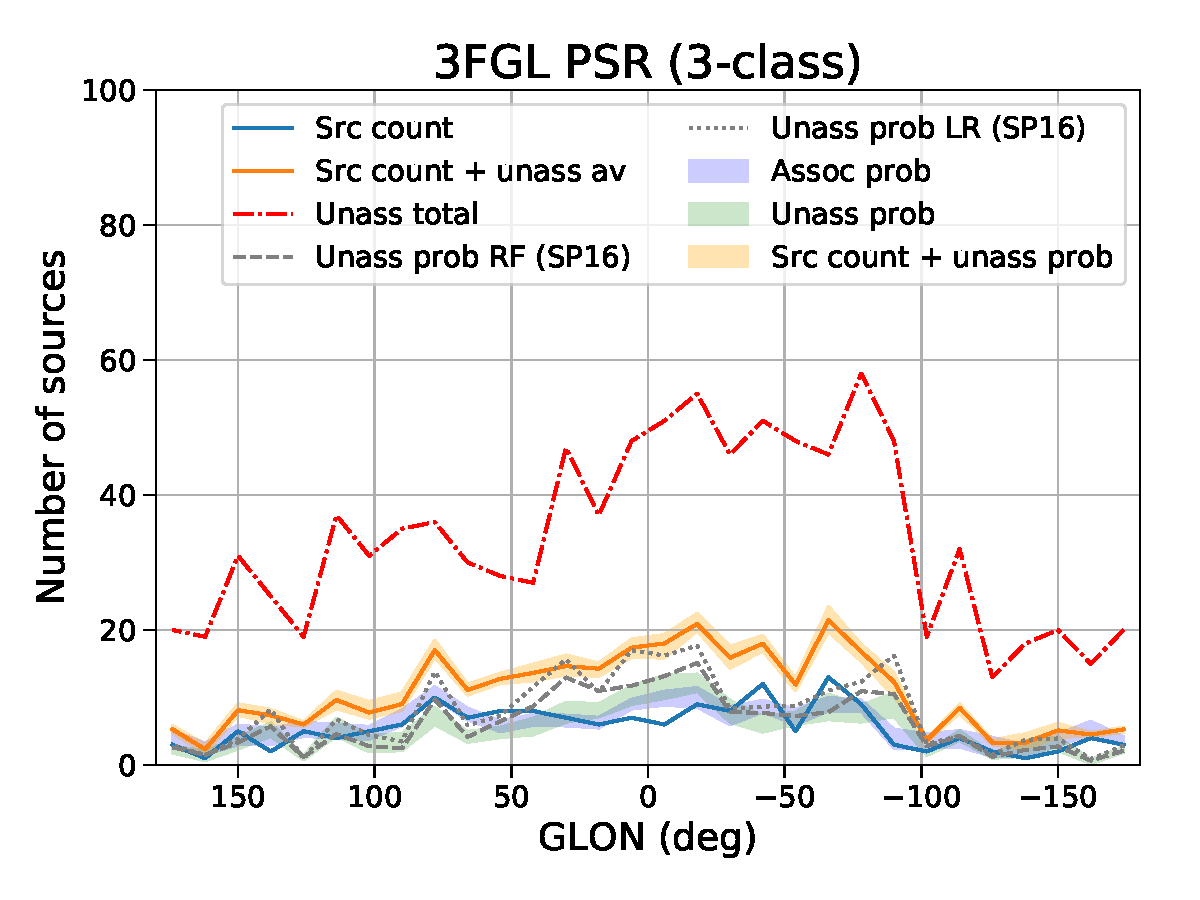
\includegraphics[width=0.45\textwidth]{plots/lon_profile_PSR_3FGL_3classes.pdf}
%\hspace*{-1cm}
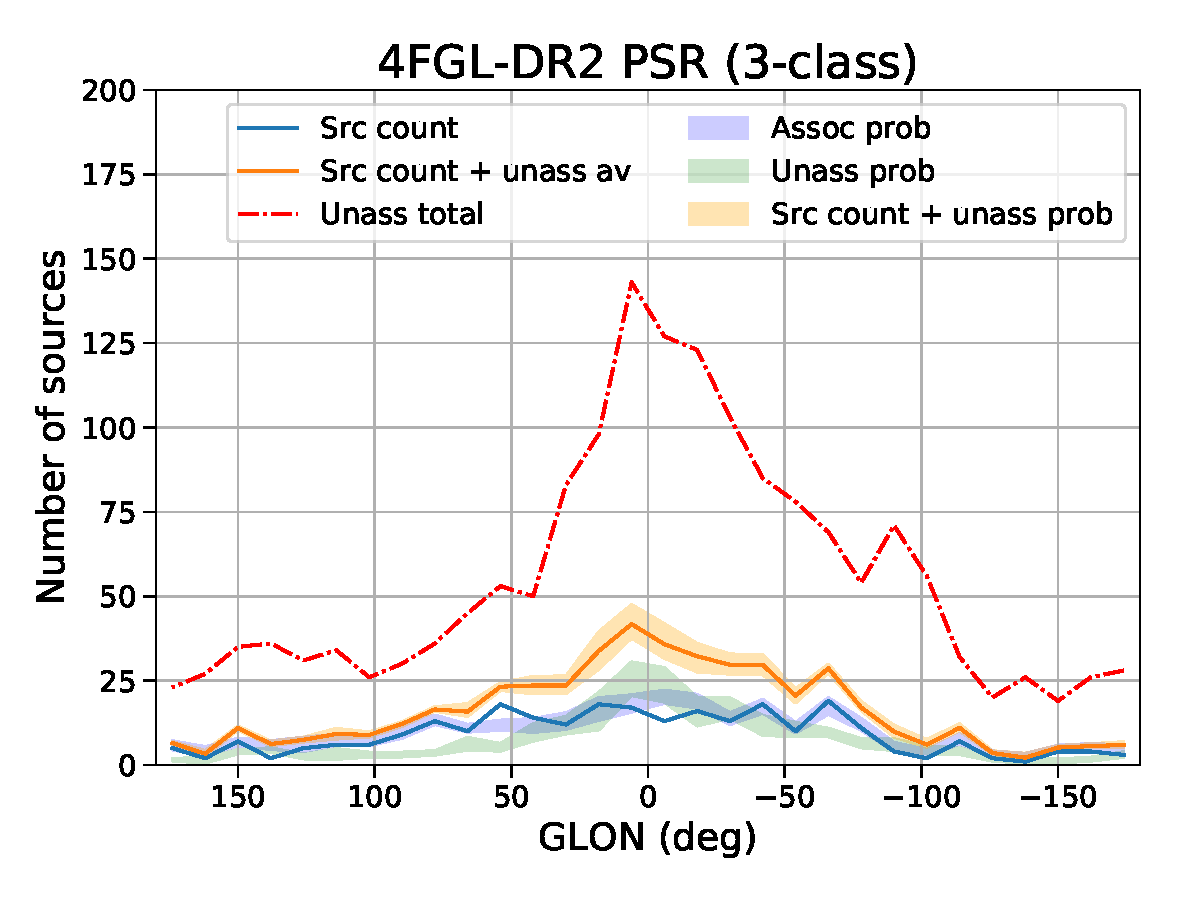
\includegraphics[width=0.45\textwidth]{plots/lon_profile_PSR_4FGL-DR2_3classes.pdf} \\
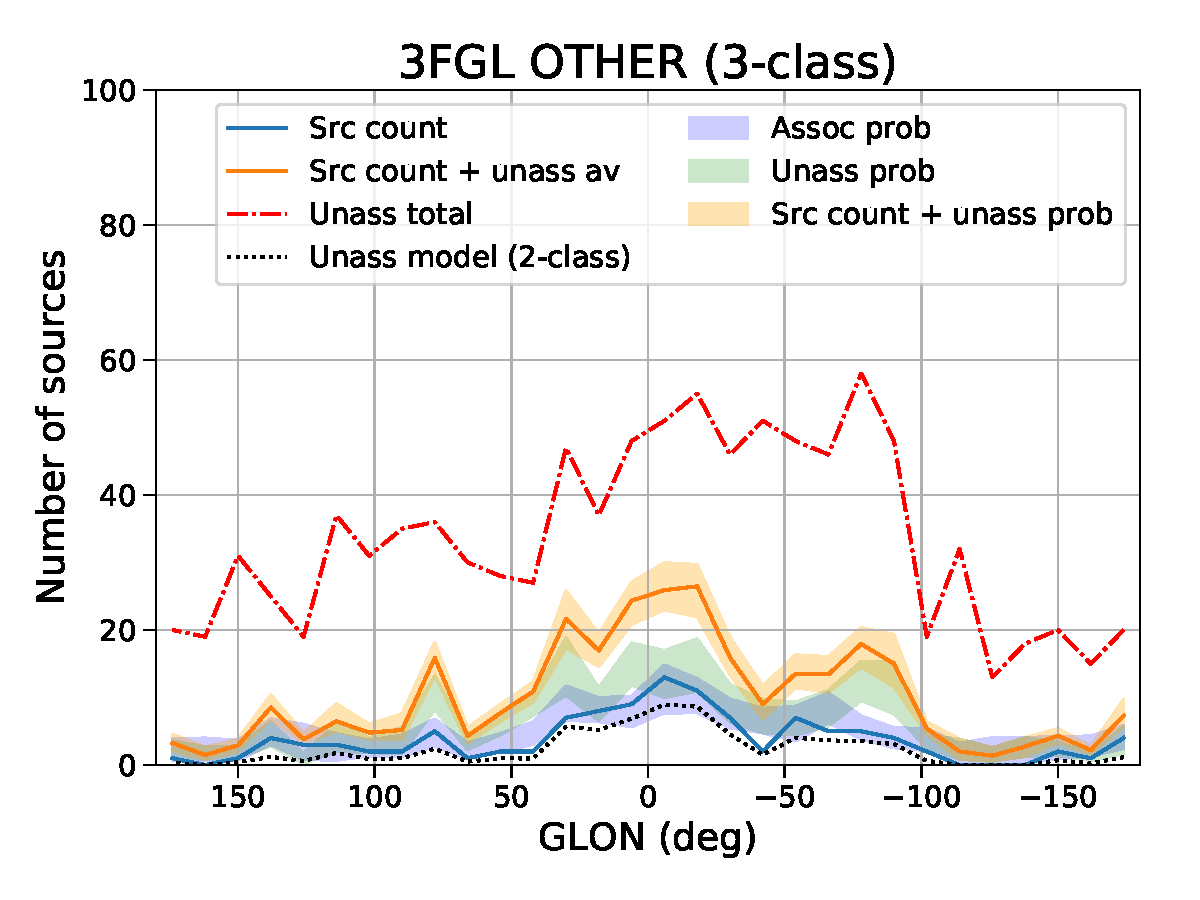
\includegraphics[width=0.45\textwidth]{plots/lon_profile_OTHER_3FGL_3classes.pdf}
%\hspace*{-1cm}
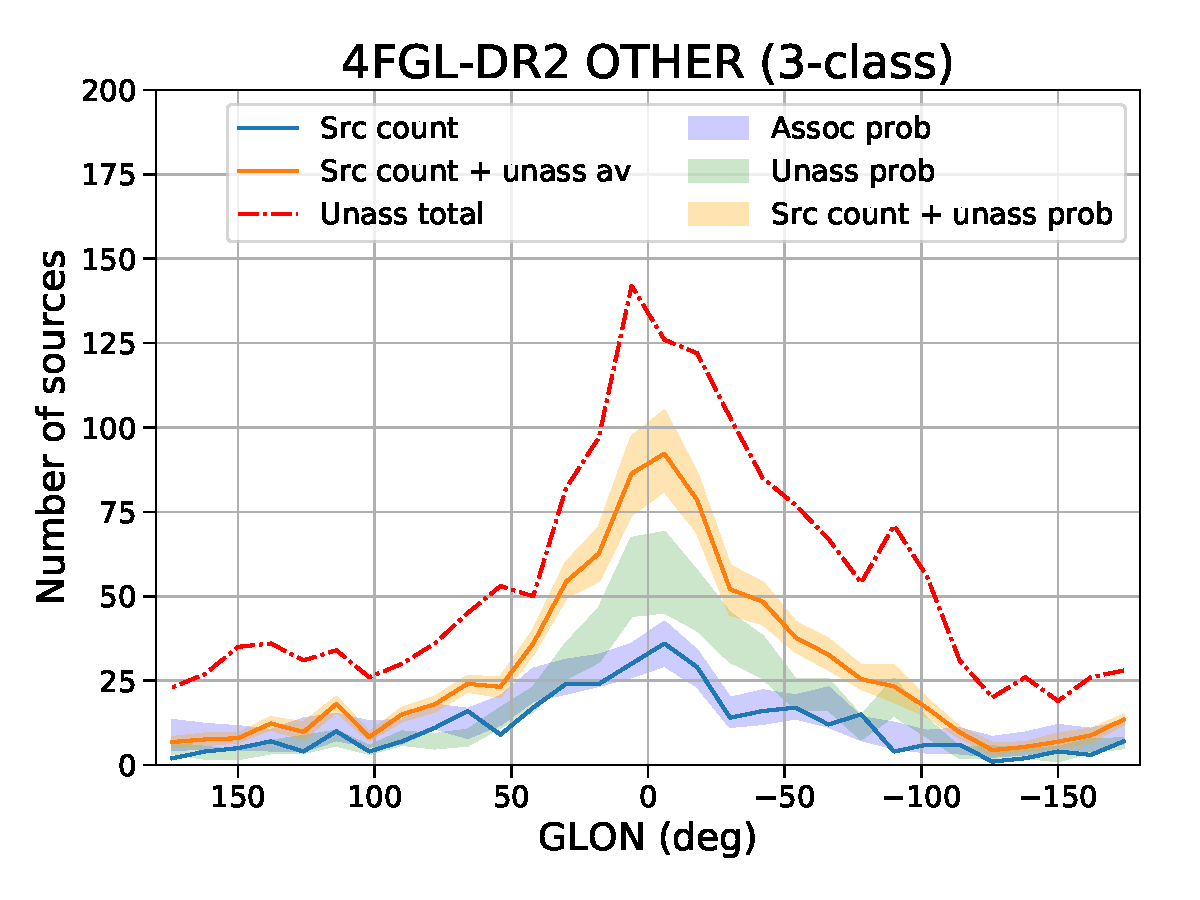
\includegraphics[width=0.45\textwidth]{plots/lon_profile_OTHER_4FGL-DR2_3classes.pdf} \\
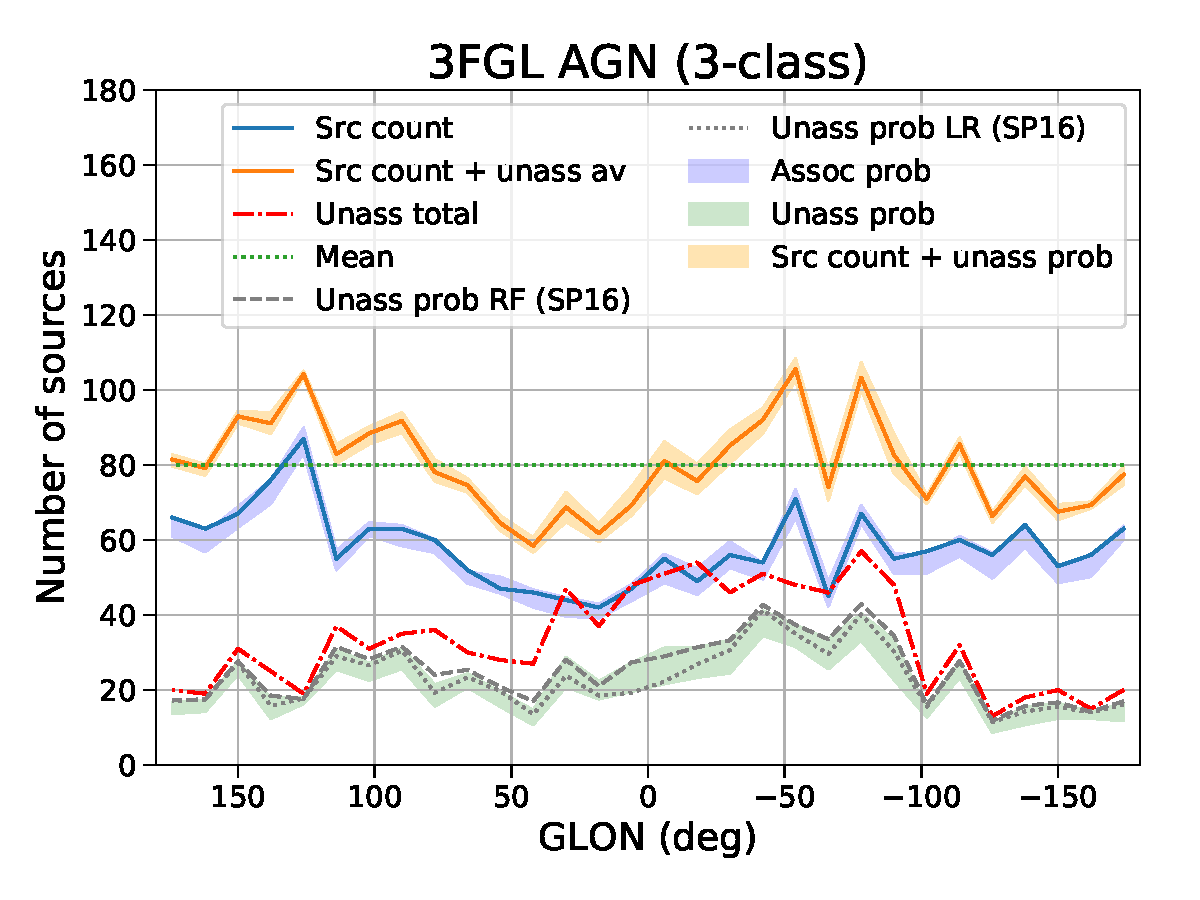
\includegraphics[width=0.45\textwidth]{plots/lon_profile_AGN_3FGL_3classes.pdf}
%\hspace*{-1cm}
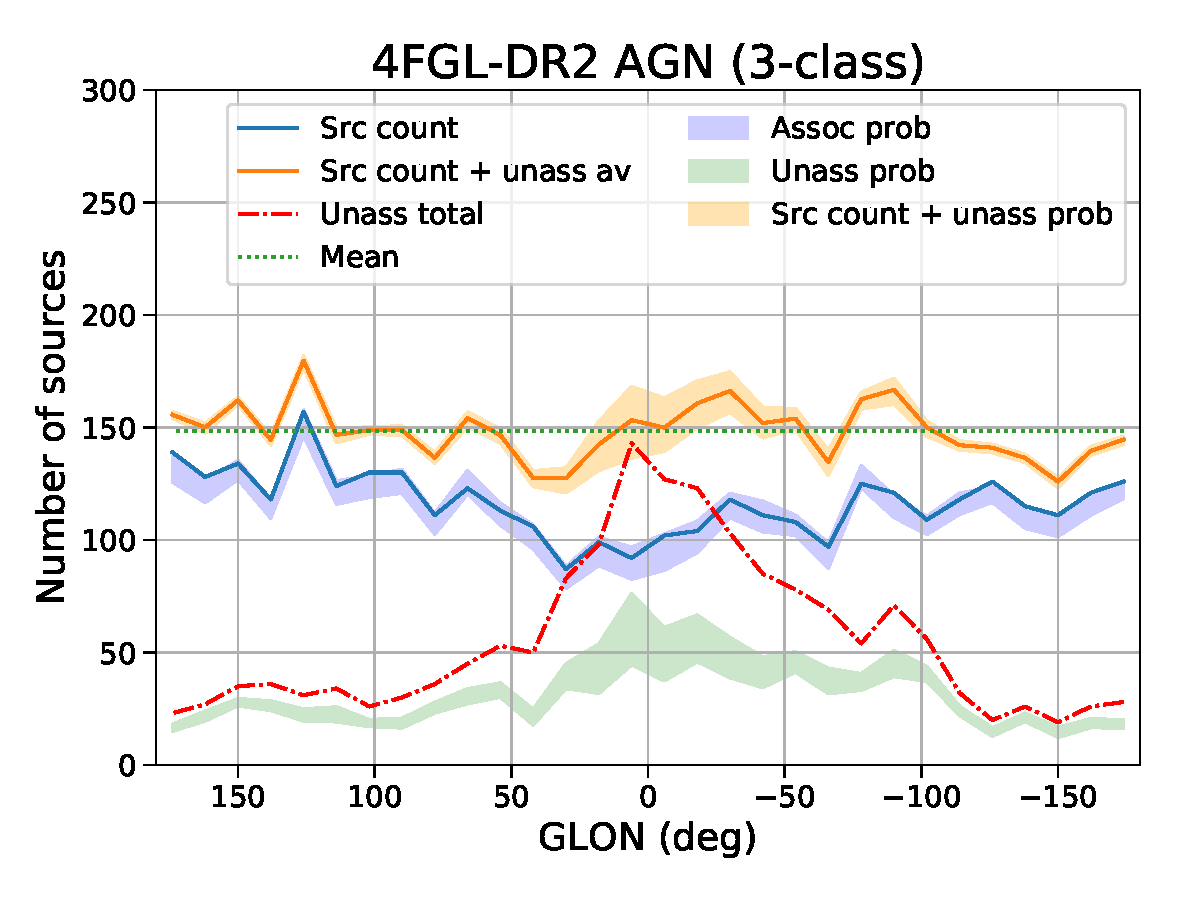
\includegraphics[width=0.45\textwidth]{plots/lon_profile_AGN_4FGL-DR2_3classes.pdf}
\caption{Longitude profiles of source counts in case of 3-class classification. For the definition of labels see Figure \ref{fig:lat_profile}.}  
\label{fig:lon_profile_3class}
\end{figure*}


In this section we show Galactic latitude and longitude profiles of the distributions of associated and unassociated sources.
In Figures \ref{fig:lat_profile} and \ref{fig:lat_profile_3class} we present the source counts as a function of ${\rm abs(sin(GLAT))}$ 
for 2-class and 3-class classifications respectively.
We use 20 bins, i.e., each bin corresponds to a solid angle of $4 \pi / 20$. 
Solid blue lines show counts of associated sources in 3FGL and 4FGL-DR2  catalogs.
It is interesting to note that the density of associated AGNs is decreasing towards the Galactic plane.
The total counts of unassociated sources are shown by red dash-dotted lines.
Green bands show the envelopes of sums of probabilities for AGN, PSR, and, in case of 3 classes, OTHER sources for the eight ML methods corrected in the case of 2 classes for the presence of OTHER sources.
Black dashed line in plots of the OTHER class show the model for the number of OTHER sources among the unassociated ones
in Equation (\ref{eq:unas_other}) for latitude bins.
We see that in the latitude profile, the 2-class model for the contribution of OTHER sources to the unassociated ones is generally consistent with the estimate of the number of OTHER sources in the 3-class model.

The classifications of unassociated 3FGL sources by \cite{2016ApJ...820....8S} are shown by gray dashed (RF) and dotted (LR) lines.
The numbers of unassociated sources classified as AGN, PSR, or OTHER grow towards the Galactic plane (GP).
Within $\approx 3^\circ$ from the GP the expected number of PSRs is about the same as the number of AGNs among unassociated sources, while at high latitudes, most of unassociated sources are classified as AGNs.
It is interesting to note, that according to Table \ref{tab:feat_imp}, GLAT is one of the least important features for the RF algorithm.
It can be a posteriori explained by the fact that the density of AGNs is such that even in the GP the expected number of AGNs is comparable to the expected number of PSRs.

Orange shaded areas show the sum of the source counts and the expected number of sources for the eight methods (both with and without oversampling).
The average among the eight methods added to the counts of associated sources is shown by solid orange line 
(for AGNs we also show the mean of these points by dotted green line).
We find that the number of associated AGNs is decreasing towards the GP, the expected number of AGNs among unassociated sources is increasing towards the GP, so that the sum of the two is relatively uniform as a function of Galactic latitude.


In Figures \ref{fig:lon_profile} and \ref{fig:lon_profile_3class} we show plots analogous to Figures \ref{fig:lat_profile} and \ref{fig:lat_profile_3class} for Galactic longitudes (we use 30 bins).
We note that there is a significant increase in the number of unassociated sources in the 4FGL-DR2  catalog for $|\ell | \lesssim 50^\circ$.
In the 2-class classification about half of the unassociated sources are attributed to pulsars and half to AGNs.
In the 3-class classification at least one third of the unassociated sources in this range of longitudes is attributed to the OTHER class.
This comes mostly at the expense of reducing the predicted number of pulsars.
It is interesting to note that the 2-class model for the OTHER sources calculated using Equation (\ref{eq:unas_other}) for longitude bins
(black dashed line in the OTHER plots) is significantly below the bands of 3-class expectations, whereas for the latitude bins the 2-class model
was consistent with the bands.
The reason is that the ratio of unassociated to associated sources, which we use to estimate the number of OTHER sources among the unassociated ones, depends on binning.
In particular, this ratio is about 1 for low latitudes, which leads to an estimate that at low latitudes the number of OTHER sources among unassociated ones is similar to the number of associated OTHER sources.
But for longitude and flux binning the ratio of unassociated to associated sources is smaller than 1, which leads to a prediction (in the 2-class case) that the number of OTHER sources among unassociated ones is smaller than the number of associated OTHER sources.

We summarize the expected numbers of sources in 2-class and 3-class models in Table \ref{tab:expected_counts_prob_3FGL} for 3FGL and in Table \ref{tab:expected_counts_prob_4FGL-DR2} for 4FGL-DR2 catalogs.
In the 2-class case we also show the correction for the presence of OTHER sources among unassociated ones.
We make the correction using the total numbers of unassociated and associated sources, as well as binning in flux from Figure \ref{fig:logN_logS} (F-bins), in latitudes from Figure \ref{fig:lat_profile} (Lat-bins), and in longitudes from Figure  \ref{fig:lon_profile}.
We see that predictions for the numbers of sources using latitude binning in the 2-class case is closest to the 3-class case.
Even better agreement would likely be achieved if ones uses a simultaneous binning in flux, latitudes, longitudes and, possibly, other variables.
If, in addition, one allows bins of variable size and non-rectangular boundaries in multi-dimensional space, then one will eventually end up with one of the ML algorithms for classification.
Indeed, ML algorithms are designed to provide an optimal binning, which maximizes the separation of classes and make predictions for data with unknown labels (e.g., unassociated sources) based on counts of samples in bins with known labels (e.g., associated sources).
Thus the 3-class prediction for classification of unassociated sources is likely more accurate than the 2-class classification with correction for OTHER sources based on ad hoc binning of one of the variables.
The 2-class classification may still be useful in situations, when high recall is necessary for either pulsars or AGNs.
Since OTHER sources are mixed with pulsars and AGNs, some of pulsars and AGNs can be mistakenly classified as OTHER in the 3-class case.




\begin{table}[!h]
%\hspace{-0.2cm}
\resizebox{0.47\textwidth}{!}{
%\tiny
\centering
%\renewcommand{\tabcolsep}{0.4mm}
%\renewcommand{\arraystretch}{1.6}

%\hspace{-3mm}
\begin{tabular}{| l |c|c|c|}
\hline
Classification &  AGN & PSR & OTHER \\
\hline
2-class  & $738.3^{+75.8}_{-97.6}$ & $269.7^{+97.6}_{-75.8}$ & --  \\
\hline
2-class corr total  & $710.6^{+69.4}_{-91.9}$ & $243.3^{+91.9}_{-69.4}$ & 54.1 \\
\hline
2-class corr F-bins  & $715.8^{+70.3}_{-93.1}$ & $252.0^{+93.1}_{-70.3}$ & 40.2 \\
\hline
2-class corr Lat-bins  & $670.1^{+67.2}_{-83.4}$ & $198.9^{+83.4}_{-67.2}$ & 139.0 \\
\hline
2-class corr Lon-bins   & $704.7^{+68.6}_{-90.7}$ & $236.0^{+90.7}_{-68.6}$ & 67.3 \\
\hline
3-class   & $662.2^{+74.9}_{-65.3}$ & $158.3^{+22.3}_{-23.6}$ & $187.5^{+46.3}_{-51.3}$ \\
\hline
\end{tabular}}
\vspace{2mm}
\caption{Expected counts of sources among unassociated 3FGL sources.}
\label{tab:expected_counts_prob_3FGL}
\end{table}


\begin{table}[!h]
%\hspace{-0.2cm}
\resizebox{0.47\textwidth}{!}{
%\tiny
\centering
%\renewcommand{\tabcolsep}{0.4mm}
%\renewcommand{\arraystretch}{1.6}

%\hspace{-3mm}
\begin{tabular}{| l |c|c|c|}
\hline
Classification &  AGN & PSR & OTHER \\
\hline
2-class  & $1177.5^{+173.4}_{-243.6}$ & $480.5^{+243.6}_{-173.4}$ & --  \\
\hline
2-class corr total  & $1098.0^{+158.7}_{-220.3}$ &$420.6^{+220.3}_{-158.7}$ & 139.4 \\
\hline
2-class corr F-bins  & $1096.8^{+158.4}_{-222.0}$ & $431.5^{+222.0}_{-158.4}$ & 127.7  \\
\hline
2-class corr Lat-bins  & $1008.0^{+141.4}_{-189.5}$ & $333.3^{+189.5}_{-141.4}$ & 316.7 \\
\hline
2-class corr Lon-bins   & $1074.9^{+154.1}_{-210.4}$ & $388.6^{+210.4}_{-154.1}$ & 194.5 \\
\hline
3-class   &$943.7^{+121.3}_{-134.6}$ & $214.3^{+47.2}_{-41.6}$ & $500.0^{+87.4}_{-101.2}$ \\
\hline
\end{tabular}}
\vspace{2mm}
\caption{Expected counts of sources among unassociated 4FGL-DR2 sources.}
\label{tab:expected_counts_prob_4FGL-DR2}
\end{table}









